\providecommand\classopts{}
\providecommand\geometryopts{}
\documentclass[a4paper,twoside\classopts]{memoir}
\usepackage{standalone}
\usepackage[utf8]{inputenc}
\usepackage[pass\geometryopts]{geometry}
\usepackage[british]{babel}
\usepackage{csquotes}
\usepackage[T1]{fontenc}
\usepackage{charter}
\usepackage[bitstream-charter]{mathdesign}
\usepackage[final,babel]{microtype}
\usepackage{siunitx}
\usepackage{amsmath}
\usepackage{bm}
\usepackage{mathtools}
\usepackage{subcaption}
\usepackage{xpatch}
\usepackage[
  backend=biber,
  style=authoryear-comp,
  firstinits=true,
  doi=false,
  isbn=false,
  uniquename=init,
  uniquelist=minyear,
  labeldate=true,
  maxcitenames=2,
  maxbibnames=5,
  hyperref=true]{biblatex}
\usepackage{minted}
\usepackage{booktabs}
\usepackage[hidelinks,pdfpagelayout=TwoPageRight]{hyperref}
\usepackage{blindtext}
\usepackage{xcolor}
\PassOptionsToPackage{final}{graphicx}
\usepackage{tikz}
\usetikzlibrary{arrows}

\addbibresource{journals.bib}
\addbibresource{dissertation.bib}

\setlrmarginsandblock{\spinemargin}{1in}{*}
\setmarginnotes{0in}{0in}{0in}
\checkandfixthelayout

\makeatletter
\def\hrulefill{\leavevmode\leaders \hrule height \rulethickness \hfill\kern\z@}
\makeatletter

\title{Representation of Mountains in Atmospheric Models}
\author{James Shaw}
\date{August 2014}

\makeatletter
\AtBeginDocument{
  \hypersetup{
    pdftitle = {\@title},
    pdfauthor = {\@author}
  }
}
\makeatother
\OnehalfSpacing
\makechapterstyle{mysouthall}{%
\setlength{\afterchapskip}{5\baselineskip}
\setlength{\beforechapskip}{36pt}
\setlength{\midchapskip}{\textwidth}
\addtolength{\midchapskip}{-\beforechapskip}
\renewcommand*{\chapterheadstart}{\vspace*{2\baselineskip}}
\renewcommand*{\chaptitlefont}{\huge\rmfamily\raggedright}
\renewcommand*{\chapnumfont}{\chaptitlefont}
\renewcommand*{\printchaptername}{}
\renewcommand*{\chapternamenum}{}
\renewcommand*{\afterchapternum}{}
\renewcommand*{\printchapternum}{%
\begin{minipage}[b]{\beforechapskip}
{\vspace{0pt}\chapnumfont%%%\figureversion{lining}
\thechapter}
\end{minipage}}
\renewcommand*{\printchaptertitle}[1]{%
\hfill\begin{minipage}[b]{\midchapskip}
{\vspace{0pt}\chaptitlefont ##1\par}\end{minipage}}
\renewcommand*{\afterchaptertitle}{%
\par\vspace{\baselineskip}%
\hrulefill \par\nobreak\noindent \vskip\afterchapskip}}
\chapterstyle{mysouthall}

\chapterstyle{mysouthall}
\blindmathtrue

\begin{document}
\newcommand{\TODO}[1]{\textcolor{purple}{TODO: \emph{#1}}}
\newcommand{\TODOsidenote}[1]{\footnote{\TODO{#1}}}
\newcommand{\TODOcite}{\textcolor{purple}{\textsuperscript{[citation needed]}}}
\newcommand{\trans}[1]{{#1^\star}}
\newcommand{\surface}{h}
\newcommand{\shellcmd}[1]{\texttt{#1}}
\newcommand{\diffusioncoeff}{\mathcal{D}}
\newcommand{\exner}{\Pi}
\newcommand{\courant}{\mathrm{Co}}

\newcommand{\vect}{\bm}
\newcommand{\del}{\nabla}

\begin{titlepage}
\begin{center}
\textsc{\Large University of Reading} \\[12pt]
{\Large Department of Meteorology} \\[12pt]

\includegraphics{uor-logo} \\[48pt]

\rule{\textwidth}{.4pt} \\[12pt]
{ \huge \bfseries Representation of Mountains in Atmospheric Models \\[12pt] } \rule{\textwidth}{.4pt} \\[54pt]
{\LARGE James Shaw}
\vfill
A dissertation submitted in partial fulfilment of the requirement for the degree of MSc Atmosphere Ocean and Climate \\[48pt]
{\Large August 2014}
\end{center}
\end{titlepage}


\frontmatter
\thispagestyle{plain}
\null\vfil
\begin{abstract}
\blindtext
\end{abstract}
\vfil

\cleardoublepage
\tableofcontents*

\mainmatter
\chapter{Introduction}

Orography has significant effects on local weather, creating strong downslope winds and enhancing local precipitation \autocite{barry2008}.
Large mountain ranges also affect global circulation.  A mountain acts as a barrier to air flow and, due to conservation of vorticity, meridional displacement balances vortex stretching, giving rise to planetary waves which affect the development of pressure systems \autocite{barry2008}.
The Tibetan Plateau acts as an elevated heat source, raising temperatures and humidity in summer which help to maintain the Asian monsoon \parencites{ye1981}{luo-yanai1983}.
Terrain also affects global circulation by exerting low-level drag \autocite{lott-miller1997} and transporting momentum via gravity waves \autocite{mcfarlane1987}.

To capture these effects, numerical weather prediction (NWP) models must solve the equations of motion on a grid that represents the orography.
Over flat ground the grid can be entirely regular, but in the presence of sloping terrain the grid must be modified.  There are two main approaches: either transform the grid so that its vertical layers follow the terrain, or remove all or part of grid cells that intersect with the orography.

Terrain following (TF) layers are in widespread use in operational models and are usually implemented on a rectangular computational grid, using terrain following vertical coordinates instead of Cartesian coordinates.  In this system, the terrain's influence decays with height: the bottommost layers follow the underlying surface closely while the uppermost layers are flat.

It is well-known that TF coordinates perform badly in the presence of steep orography \autocite{gary1973}.  As spatial resolution in NWP models increases, gradients in terrain tend to become steeper \autocite{steppeler2002}.  This leads to larger truncation errors in calculating the horizontal pressure gradient which result in spurious winds \autocite{dempsey-davis1998}.  Much work has been done to reduce error associated with TF coordinates: firstly, by smoothing the effects of terrain with height \parencites{simmons-burridge1981}{schaer2002}{leuenberger2010}{klemp2011} and, secondly, by improving the accuracy in calculating the horizontal pressure gradient itself \parencites{mahrer1984}{klemp2011}{zaengl2012}.

Despite their associated numerical errors, TF coordinates are attractive because their rectangular structure is simple to process by computer, boundary layer resolution can be increased with variable spacing of vertical layers \autocite{schaer2002}, and cell sizes remain almost constant \autocite{jebens2011}.

An alternative to terrain following layers is to `shave', or `cut', cells where they intersect with the terrain surface.  Cells that lie entirely below the terrain are removed, and those that intersect the surface are modified in shape so that they more closely fit the terrain.  This modification means that some cells become very small, which can reduce computational efficiency \autocite{klein2009}, and several approaches have been tried to alleviate the problem \parencites{steppeler2002}{yamazaki-satomura2010}{jebens2011}.

Several studies found that cut cells produce more accurate results when compared to TF coordinates.  Spurious winds seen in TF coordinates are not present and errors do not increase with steeper terrain \autocite{good2013}.  A comparison of TF and cut cells using real initial data by \textcite{steppeler2006} found that precipitation patterns, temperature and wind fields were forecast more accurately in the cut cell model.  

Other representations of terrain have been developed using unstructured grids \parencites{ss2011}{pain2005}.  They are able to represent the boundary accurately, but more complex discretisations are required to maintain accuracy because the mesh is not aligned with the dominant vertical force of gravity \autocite{rosatti2005}, just as horizontal pressure gradients are difficult to calculate in TF coordinates.

Unstructured grids can be combined with dynamic mesh adaptation so that small scale features can be resolved in areas of interest, such as regions of frontogenesis, inversion layers, and the boundary layer \autocite{browne2014}.  Dynamically adaptive meshes reduce the number of grid cells needed to represent small scale features, but updating the mesh can take a significant amount of computation time \parencites{blaise2012}{browne2014}.  Furthermore, mesh adaptation does not necessarily lead to a more accurate model \autocite{parkinson2014}.

\section*{Project outline}
This project aims to compare the accuracy of TF and cut-cell style grids in a variety of two-dimensional test cases.   Simulations are performed using the OpenFOAM CFD library \autocite{openfoam} with a finite volume discretisation of the fully compressible Euler equations from \textcite{weller-shahrokhi2014}.  The model includes a curl-free pressure gradient formulation, an upwind-biased cubic advection scheme, and a Lorenz vertical staggering of variables.  All tests are performed using the same model on TF and cut cell style grids, enabling like-for-like comparison between grids.

In chapter~\ref{sec:theory}, the theory of coordinate transforms is introduced and applied to a discretisation of the horizontal pressure gradient.  We review the main types of terrain following transformations and present three shaving techniques used to construct cut cell grids.  The finite volume method, grid skewness, and the Lorenz and Charney--Phillips vertical staggerings are outlined.  We end the chapter with a brief description of the linear theory of gravity waves that is later used to evaluate experimental results.

In chapter~\ref{sec:method}, we describe the method of grid construction using the OpenFOAM CFD library.  An overview of the model discretisation from \textcite{weller-shahrokhi2014} is given and its curl-free pressure gradient and upwind-biased cubic advection scheme are described.  The chapter concludes by describing the calculation of energy measures and the Courant--Friedrichs--Lewy criterion on an unstructured grid.

The results of five experiments are discussed in chapter~\ref{sec:results}.  Results of three standard test cases are compared with results from the literature, and two new test cases are developed which shed light on some problems with cut cells.  The first two tests challenge the upwind-biased advection scheme.  The first, standard test transports a tracer in a horizontal flow.  The second test is formulated to find the cause of errors in the horizontal advection test by transporting a tracer in a terrain following flow.  The third test examines spurious motion in a resting atmosphere in the presence of orography.  The fourth test generates orographically induced gravity waves and errors in potential temperature found on the cut cell style grid are discussed.  A final test is developed to investigate the cause of these errors by advecting a stable thermal profile.

Concluding remarks on the experimental results are made in chapter~\ref{sec:conclusions}.  Finally, areas of further work are discussed in chapter~\ref{sec:further-work}.  Additional tests are suggested to explore the source of numerical errors that were found in the experimental results.  In particular, we recommend the formulation of a new Charney--Phillips staggering on unstructured grids.  We hope that, by modifying the model to use this staggering, numerical error would be reduced.

\chapter{Theoretical basis}
\label{sec:theory}
\TODO{repeat some of the intro to TF layers from previous chapter}

In this chapter, we present the theory of coordinate transformation and demonstrate how it can be applied to a forward-in-space discretisation of a horizontal pressure gradient.  We go on to review the origins of terrain following coordinates and more recent refinements to terrain following grids.  Next, the cut cell method is described.  We outline the `small cell' problem that is inherent with the cut cell method and explain some approaches that address it.

After outlining the finite volume discretisation method that is used by the model for this project, we discuss the two most common vertical staggerings of variables: the Charney--Phillips grid and the Lorenz grid.  The chapter concludes with a review of linear wave theory, giving examples of the structure of stationary waves over infinite sinusoidal hills.

\section{Coordinate transformations}
\label{sec:theory:coord-transform}

A model implementation that uses terrain following layers must first choose from a variety of vertical coordinates.  The equations of motion with the hydrostatic approximation are simplified by using pressure coordinates \autocite{eliassen1949}.  However, because pressure varies in the horizontal, the lower boundary condition becomes complicated because surfaces of constant pressure intersect the terrain.  This motivated \textcite{phillips1957} to create the sigma coordinate in which pressure is normalised such that $\sigma$ ranges between zero at the top of the domain, and one at the surface.
Most hydrostatic models use normalised pressure coordinates.  With some exceptions, such as \textcite{xue-thorpe1991}, nonhydrostatic models use height-based coordinates \autocite{steppeler2003}.

Isentropic coordinates have also been investigated.  Since adiabatic motion follows isentropic surfaces, errors in discretising vertical advection are negligible.  However, difficulties arise when isentropes intersect with the surface \autocite{konor-arakawa1997}.

Second, a model may choose to use transformed coordinates.  Typically, terrain following models use transformed height or pressure coordinates so that the computational domain becomes rectangular.
Consider the two-dimensional Cartesian coordinates $(x, z)$ and transformed coordinates $(\trans{x}, \trans{z})$ which must be a monotonic function of $z$ so that the transformation is invertible.

A scalar field, $\varphi$, can be expressed in transformed coordinates as $\varphi(\trans{x}, \trans{z})$ or in Cartesian coordinates as $\varphi(\trans{x}(x), \trans{z}(x, z))$.
Hence the vertical derivative of $\varphi$ can be found by using the chain rule \autocite{mit2004}
\begin{align}
  \frac{\partial \varphi}{\partial z} =
  \frac{\partial \varphi}{\partial \trans{z}}
  \frac{\partial \trans{z}}{\partial z} \label{eqn:theory:grad-transform}
\end{align}

The multivariable chain rule is needed to find the horizontal derivative.  Given two sets of functions
\begin{align*}
	y_1 &= y_1(u_1, \dots, u_j) \quad \\
	    &\vdots \\
	y_i &= y_i(u_1, \dots, u_j)
%
	\intertext{and}
%
	u_1 &= u_1(x_1, \dots, x_k) \\
	    &\vdots \\
	u_j &= u_j(x_1, \dots, x_k)
%
\end{align*}
we can apply a $i \times k$ Jacobi rotation matrix
\begin{align}
\frac{\partial y_i}{\partial x_k} = 
\begin{bmatrix}
  \dfrac{\partial y_1}{\partial x_1}	& \dfrac{\partial y_1}{\partial x_2} &	\cdots &	\dfrac{\partial y_1}{\partial x_k} \\
  \vdots				& \vdots &				\ddots &	\vdots \\
  \dfrac{\partial y_i}{\partial x_1}	& \dfrac{\partial y_i}{\partial x_2} &	\cdots &	\dfrac{\partial y_i}{\partial x_k}
\end{bmatrix}
%
\intertext{where $y_i$ is a first-order tensor with $i$ covariant indices.  Similarly, defining the tensors $\partial y_i / \partial u_j$ and $\partial u_j / \partial x_k$ then we can express the chain rule as}
%
\frac{\partial y_i}{\partial x_k} = \frac{\partial y_i}{\partial u_j} \frac{\partial u_j}{\partial x_k}
%
\intertext{Applying this to $\varphi$ we find}
%
\begin{bmatrix}
	\frac{\partial \varphi}{\partial x}  &  \frac{\partial \varphi}{\partial z}
\end{bmatrix}
=
\begin{bmatrix}
	\frac{\partial \varphi}{\partial \trans{x}}  &  \frac{\partial \varphi}{\partial \trans{z}}
\end{bmatrix}
\begin{bmatrix}
	\frac{\partial \trans{x}}{\partial x} & 	\frac{\partial \trans{x}}{\partial z} \\
	\frac{\partial \trans{z}}{\partial x} &	\frac{\partial \trans{z}}{\partial z}
\end{bmatrix} \label{eqn:theory:transform-matrix}
%
\intertext{and the horizontal component of equation~\ref{eqn:theory:transform-matrix} is then}
%
\left. \frac{\partial \varphi}{\partial x} \right|_z =
\left. \frac{\partial \varphi}{\partial \trans{x}} 
	\frac{\partial \trans{x}}{\partial x} \right|_\trans{z} +
	\frac{\partial \varphi}{\partial \trans{z}}
	\left. \frac{\partial \trans{z}}{\partial x} \right|_z \label{eqn:theory:coord-trans-hv}
%
	\intertext{where the subscript by the vertical bar denotes the variable that is held constant.  When there is no transformation of horizontal coordinates, $x = \trans{x}$, and equation~\ref{eqn:theory:coord-trans-hv} simplifies to}
%
\left. \frac{\partial \varphi}{\partial x} \right|_z =
\left. \frac{\partial \varphi}{\partial \trans{x}} \right|_\trans{z} +
	\frac{\partial \varphi}{\partial \trans{z}}
	\left. \frac{\partial \trans{z}}{\partial x} \right|_z \label{eqn:theory:coord-trans}
\end{align}

In a two-dimensional terrain-following coordinate transform, there is the added requirement that the transformed domain be rectangular.  This can be satisfied by imposing boundary conditions \autocite{schaer2002}
\begin{align}
	\trans{z}(x, \surface(x)) = 0 \quad,\quad \trans{z}(x, H) = H
\end{align}
where $H$ is the height of the domain and $h(x)$ is the height of the terrain surface.

\section{Horizontal pressure gradient}
In models that use TF coordinates, the horizontal pressure gradient can be calculated in the transformed coordinate system.  It follows from equation~\ref{eqn:theory:coord-trans} that, in TF coordinates, the horizontal gradient of pressure $p$ is \autocite{mahrer1984}
\begin{align}
	\left. \frac{\partial p}{\partial x} \right|_z = 
	\left. \frac{\partial p}{\partial x} \right|_\trans{z} + 
	\left. \frac{\partial \trans{z}}{\partial x} \right|_z
	\frac{\partial p}{\partial \trans{z}} \label{eqn:theory:pressure-transform}
\end{align}
The first term on the right hand side is the change in pressure along the TF coordinate surface, and the second term corrects for the vertical variation in the first.  These terms tend to be large and of opposite sign over steep terrain, and a discretisation must be at least first order accurate so that the difference between the hydrostatic components of the two terms converges to zero \autocite{gary1973}.

A first-order forward difference approximation of the horizontal pressure gradient can be found from equation~\ref{eqn:theory:pressure-transform}, such that
\begin{align}
	\left. \frac{\partial p}{\partial x} \right|_z &= \frac{p_{i+1,k} - p_{i,k}}{\Delta x} + \frac{\partial \trans{z}}{\partial x} \frac{p_{i+1,k} - p_{i+1,k-1}}{\Delta \trans{z}} + \mathcal{O}(\Delta x)
\end{align}

Errors in the horizontal pressure gradient are associated with horizontal acceleration by the momentum equation, and have been shown to generate spurious winds \parencites{klemp2003}{klemp2011}.

Errors can be reduced by improving the accuracy of the horizontal pressure gradient discretisation.  \textcite{mahrer1984} proposed a discretisation where two pressure values at the same geometric height are interpolated from surrounding points.  From these values, a horizontal pressure gradient can be calculated without introducing metric terms.  Recent studies have found that variations of Mahrer's technique reduce spurious circulations \parencites{dempsey-davis1998}{klemp2011}{zaengl2012}.  \TODO{does this imply approach without metric terms is better than with?  can this be justified?}

\section{Terrain following techniques}
\label{sec:theory:tf}

\begin{figure}
	\captionsetup[subfigure]{position=b}
	\centering
	\subcaptionbox{Basic terrain following (BTF) \label{fig:intro:tf:btf}}[0.45\textwidth]{\input{btf-plot}}
	\hfill
	\subcaptionbox{Smooth level vertical (SLEVE) \label{fig:intro:tf:sleve}}[0.45\textwidth]{\input{sleve-plot}}
	\caption{Example vertical cross sections of terrain following layers illustrating the decay in terrain influence with height.   In BTF the decay is linear; in SLEVE it is exponential.}
	\label{fig:intro:tf}
\end{figure}

As well as improving discretisation accuracy, errors due to coordinate transformation can also be reduced by smoothing the effect of the terrain so that the grid becomes more regular aloft. 

\textcite{galchen-somerville1975} proposed a basic terrain following (BTF) coordinate system in which the terrain's influence decays linearly with height but disappears only at the top of the domain (example shown in figure~\ref{fig:intro:tf:btf}).  The transformation is defined as
\begin{align}
	\trans{z} &= H \frac{z - \surface}{H - \surface} \label{eqn:theory:btf}
%
\intertext{or}
%
	z &= \left( H - \surface \right) \frac{\trans{z}}{H} + \surface
\end{align}
where, in two dimensions, $z(x, \trans{z})$ is the height of the coordinate surface at level $\trans{z}$, $H$ is the height of the domain, and $\surface(x)$ is the height of the terrain surface.

The sigma coordinate transform of \textcite{phillips1957} is equivalent to the BTF coordinate transform since they both decay linearly.  However, since they decay with pressure rather than height, sigma coordinates also change with horizontal variations in pressure.

The hybrid terrain following (HTF) coordinates of \textcite{simmons-burridge1981} improve upon BTF coordinates by allowing the vertical decay profile can be controlled.  By choosing a suitable profile, terrain influence decays more rapidly than BTF to produce surfaces of constant height aloft \autocite{klemp2011}.

The coordinate system can be further refined by decaying small-scale features more rapidly than large-scale features to produce smooth coordinate surfaces in the middle and top of the domain.
\textcite{schaer2002} achieved this with smooth level vertical (SLEVE) coordinates in which terrain height is split into a large-scale component $\surface_1$ and a small-scale component $\surface_2$ such that $\surface = \surface_1 + \surface_2$.  Each component has a different exponential decay profile.  The transformation is defined as
\begin{align}
	z &= \trans{z} + \surface_1 b_1 + \surface_2 b_2
%
\intertext{with the vertical decay functions are given by}
%
	b_i &= \frac{\sinh \left( \left( H - \trans{z} \right) / s_i \right)}{\sinh \left( H / s_i \right)}
\end{align}
where $s_1$ and $s_2$ are the scale heights of large-scale and small-scale terrain respectively.  SLEVE produces smooth coordinate surfaces in the middle and top of the domain (see figure~\ref{fig:intro:tf:sleve}).

\textcite{leuenberger2010} generalised the SLEVE transformation in order to increase cell thickness in the layers nearest the ground, allowing longer timesteps and permitting more accurate calculation of parameterised low-level heat and momentum fluxes.  An exponent $n$ is introduced so that the generalised decay functions become
\begin{align}
	b_i &= \frac{\sinh \left( \left( H / s_i \right)^n - \left( \trans{z} / s_i \right)^n \right)}{\sinh \left( H / s_i \right)^n}
\end{align}
where the optimal exponent value was found to be $n = 1.35$.

In the smoothed terrain following (STF) coordinate, \textcite{klemp2011} took an alternative approach, using a multipass smoothing operator, and found that errors were reduced still further compared to SLEVE.


\section{Cell shaving techniques}
\label{sec:theory:shaving}

\begin{figure}
	\captionsetup[subfigure]{position=b}
	\centering
	\subcaptionbox{Full-step \label{fig:intro:shaved:full}}[0.32\textwidth]{\input{full-step-plot}}
	\subcaptionbox{Partial-step \label{fig:intro:shaved:partial}}[0.32\textwidth]{\input{partial-step-plot}}
	\subcaptionbox{Piecewise linear.  Grid boxes marked with asterisk ($\ast$) denote small cells. \label{fig:intro:shaved:piecewise-linear}}[0.32\textwidth]{\input{cut-cell-plot}}
	\caption{Vertical cross sections illustrating different methods of shaving cells intersecting with a hypothetical surface (heavy line).  Adapted from \textcite{adcroft1997}.}
	\label{fig:intro:shaved}
\end{figure}

\textcite{mesinger1988} proposed a grid that, like terrain following grids, retains almost-constant cell sizes.  The step-mountain (or `full-step') coordinate removes cells that are intersected by the terrain so creating steps over the surface (see figure~\ref{fig:intro:shaved:full}).  \textcite{gallus-klemp2000} found that lee slope winds are too weak over smooth orography, but this study did not examine performance over steep terrain.  In contrast, \textcite{mesinger2004} compared results from three operational NCEP models that suggested the step-coordinate model was more skillful than the TF coordinate models in forecasting precipitation over the mountainous western United States.

\textcite{adcroft1997} proposed a partial-step system for modelling the ocean surface in which the cell height is adjusted so that cell volume is accurately represented (figure~\ref{fig:intro:shaved:partial}).  Compared to the full-step approach of \textcite{mesinger1988}, spurious oscillations were significantly reduced advecting a tracer over topography.

The piecewise linear cut cell method is another alternative to terrain following layers.  Here, the surface terrain is intersected with a regular Cartesian grid such that cells are cut where they intersect with the ground (see figure~\ref{fig:intro:shaved:piecewise-linear}).  
This leads to cells that are entirely above the surface, entirely below it, and those which intersect with the ground.  Those cells which intersect the ground have, in two dimensions, a triangular, trapezoidal or pentagonal shape \autocite{rosatti2005}.  Figure~\ref{fig:intro:shaved:piecewise-linear} shows an example of this method.  In some grid boxes, small cells, marked with an asterisk ($\ast$), are created by intersection with the surface.
The primary difficulty is with numerical stability and reduced model efficiency associated with small cells. \TODOsidenote{also, vertical resolution varies at mountain top, leads to only 1st order accuracy for 2nd order schemes... need to find citation}

A variety of solutions to the `small cell problem' have been proposed.  In \textcite{yamazaki-satomura2010}, small cells are combined with horizontally or vertically adjacent cells.  \textcite{steppeler2002} use a `thin-wall' approximation to increase the computational volume of small cells without altering the terrain.  Conceptually, each cell partially or completely below the mountain is filled with air and surrounded by a thin wall.  Where a cell is cut by the terrain, the computational volume is equal to that of an uncut cell.  \textcite{jebens2011} avoid the timestep restriction associated with explicit schemes by using an implicit method for cut cells and a semi-explicit method elsewhere.


\section{Finite volume method}
\label{sec:theory:fv}

The finite volume method is a discretisation technique that represents the spatial domain as a non-overlapping grid of cells with fields represented as piecewise constant in each cell.  At each timestep, cell averages are updated by considering the flux $\vect{F}$ across the faces of the cell surface.  In atmospheric modelling, $\vect{F}$ is typically the advective flux $\vect{u} \varphi$ where $\vect{u}$ is the velocity field.

The notation used in this project for the representation of discrete variables follows \textcite{weller-shahrokhi2014}.  A cell average of $\varphi$ is written as $\varphi_c$, where $c$ denotes a cell.  A scalar field, $\psi$, located at a face is written as $\psi_f$, where $f$ denotes a cell face.  An interpolation of cell centre averages of $\varphi$ onto a face $f$ is written as $\varphi_F$.  $f \in \: c$ represents the faces of a cell.  $c \in \: f$ represents the cells $c$ that share a face $f$.

To describe the finite volume method, we start by considering the conservation of $\varphi$
\begin{align}
	\frac{\partial \varphi}{\partial t} + \del \cdot \left( \vect{u} \varphi \right) = 0
%
\intertext{Taking the volume integral over a cell $c$ with volume $V_c$ we find}
%
	\int_{V_c} \frac{\partial \varphi}{\partial t} \diff V + \int_{V_c} \del \cdot \left( \vect{u} \varphi \right) \diff V &= 0
%
\intertext{Integrating the first term gives the cell average $\varphi_c$ and applying the divergence theorem to the second term gives a surface integral, hence}
%
	V_c \frac{\partial \varphi_c}{\partial t} + \int_{S_c} \varphi \vect{u} \cdot \nunit \diff S &= 0
%
\intertext{where $S_c$ is the cell surface area and $\nunit$ is the unit vector that is outward normal to the surface.  Dividing by the cell volume and, for a cell with a finite number of surfaces, this becomes}
%
	\frac{\partial \varphi_c}{\partial t} + \frac{1}{V_c} \sum_{f \in \: c} \varphi_F \vect{u}_f \cdot \nunit S_f &= 0 \label{eqn:theory:discrete-continuity}
\end{align}
where $S_f$ is the surface area of face $f$, and $\varphi_F$ is the interpolated value of $\varphi$ at the face.  This interpolation of cell averages onto faces is a significant source of truncation error in finite volume systems \autocite{adcroft1997}.

The finite volume method often leads to a staggering of variables with fluxes at cell faces similar to an Arakawa C grid.  Because cell averages are modified only through surface fluxes, a quantity of $\varphi$ the fluxes out of one cell must flux into another.  Thus, $\varphi$ is conserved in the finite volume method.

\section{Vertical staggering of variables}
\label{sec:theory:staggering}

\TODO{if this section is staying in Theory chapter, make sure you define variables here and you can skip some of them in Discretisation of Euler equations later on}

\begin{figure}
	\centering
	\documentclass[tikz]{standalone}
\usepackage{bm}
\usetikzlibrary{patterns}
\newcommand{\vect}{\bm}
\newcommand{\del}{\nabla}

\newcommand{\trans}[1]{{#1^\star}}
\newcommand{\surface}{h}
\newcommand{\shellcmd}[1]{\texttt{#1}}
\newcommand{\diffusioncoeff}{\mathcal{D}}
\newcommand{\exner}{\Pi}
\newcommand{\courant}{\mathrm{Co}}

\begin{document}
\begin{tikzpicture}[
  scale=0.7
]
\fill [pattern=north west lines] (0,0) rectangle (6,-0.4);
\fill [pattern=north west lines] (8,0) rectangle (14,-0.4);
\node at (7,0) {$\frac{1}{2}$};
\draw [dashed] (0,0) -- (6,0) node [at start, anchor=east] {$w$};
\draw [dashed] (8,0) -- (14,0) node [at end, anchor=west] {$\theta, w$};

\node at (7,1) {$1$};
\draw (0,1) -- (6,1) node [at start, anchor=east] {$u, v, \theta, \rho, \exner$};
\draw (8,1) -- (14,1) node [at end, anchor=west] {$u, v, \rho, \exner$};

\node at (7,2) {$\frac{3}{2}$};
\draw [dashed] (0,2) -- (6,2) node [at start, anchor=east] {$w$};
\draw [dashed] (8,2) -- (14,2) node [at end, anchor=west] {$\theta, w$};

\node at (7,3) {$2$};
\draw (0,3) -- (6,3) node [at start, anchor=east] {$u, v, \theta, \rho, \exner$};
\draw (8,3) -- (14,3) node [at end, anchor=west] {$u, v, \rho, \exner$};

\node at (7,4) {$\frac{5}{2}$};
\draw [dashed] (0,4) -- (6,4) node [at start, anchor=east] {$w$};
\draw [dashed] (8,4) -- (14,4) node [at end, anchor=west] {$\theta, w$};

\node at (3,5) {$\vdots$};
\node at (11,5) {$\vdots$};

\node at (7,6) {$k - \frac{1}{2}$};
\draw [dashed] (0,6) -- (6,6) node [at start, anchor=east] {$w$};
\draw [dashed] (8,6) -- (14,6) node [at end, anchor=west] {$\theta, w$};

\node at (7,7) {$k$};
\draw (0,7) -- (6,7) node [at start, anchor=east] {$u, v, \theta, \rho, \exner$};
\draw (8,7) -- (14,7) node [at end, anchor=west] {$u, v, \rho, \exner$};

\node at (7,8) {$k + \frac{1}{2}$};
\draw [dashed] (0,8) -- (6,8) node [at start, anchor=east] {$w$};
\draw [dashed] (8,8) -- (14,8) node [at end, anchor=west] {$\theta, w$};

\node at (7,9) {$k + 1$};
\draw (0,9) -- (6,9) node [at start, anchor=east] {$u, v, \theta, \rho, \exner$};
\draw (8,9) -- (14,9) node [at end, anchor=west] {$u, v, \rho, \exner$};

\node at (7,10) {$k + \frac{3}{2}$};
\draw [dashed] (0,10) -- (6,10) node [at start, anchor=east] {$w$};
\draw [dashed] (8,10) -- (14,10) node [at end, anchor=west] {$\theta, w$};

\node at (3,11) {$\vdots$};
\node at (11,11) {$\vdots$};
\end{tikzpicture}
\end{document}

	\caption{Lorenz (left) and Charney--Phillips (right) vertical staggering of variables.  Solid lines represent full levels, dashed lines represent half levels.  Adapted from \textcite{holdaway2013}.}
	\label{fig:theory:staggering}
\end{figure}

When discretising the equations of motion, computational properties including stability and convergence are necessary.  Additionally, it is desirable to obtain a discretisation that represents the dynamics of the real system.  There are two commonly-used vertical staggerings, the Lorenz grid \autocite{lorenz1960} and the Charney--Phillips grid \autocite{charney-phillips1953}, which offer different sets of computational and physical properties.

In both grids, horizontal velocities $u$ and $v$, and density $\rho$, are stored at full levels, and the vertical velocity, $w$, is stored at half levels.  The two grids differ in their placement of potential temperature, $\theta$: on the Charney--Phillips grid it is stored at half levels, and at full levels on the Lorenz grid.  These arrangements of variables are summarised in figure~\ref{fig:theory:staggering}.

The Charney--Philips grid was originally developed for a quasigeostrophic model using sigma coordinates.  \textcite{arakawa-moorthi1988} found that advection of quasi-geostrophic potential vorticity is conserved by this grid staggering, and it requires less interpolation of variables than the Lorenz grid \autocite{holdaway2013}. \TODO{anything else of significant interest to say about it?}

The Lorenz grid has a number of diserable properties: it conserves total energy, the mean potential temperature, and variance of potential temperature assuming no diabatic processes or friction \autocite{arakawa-konor1996}.  However, it is known that a computational mode exists on the Lorenz grid which can create a zig-zag in the vertical distribution of potential temperature \parencites{arakawa-moorthi1988}{arakawa-konor1996}{holdaway2013b}.  This can be explained by considering the vertical momentum equation \autocite{holdaway2013}
\begin{align}
	\frac{\partial w}{\partial t} + \vect{u} \cdot \del w = -g - c_p \theta \frac{\partial \exner}{\partial z}
\end{align}
In a discretisation of this equation, to calculate $w_{k+\frac{1}{2}}$, $\theta_{k+\frac{1}{2}}$ may be interpolated using an arithmetic mean of the adjacent values $\theta_k$ and $\theta_{k+1}$.  As shown in figure~\ref{fig:theory:theta-oscillation}, a grid-scale vertical wave in potential temperature would not be visible by the model \autocite{holdaway2013}.

The computational mode can affect the physical mode, causing spurious interactions with condensation processes \autocite{arakawa-konor1996} and the spurious generation of baroclinic instability and increased gravity wave activity \parencites{arakawa-moorthi1988}{cullen1997}.

\begin{figure}
	\centering
	\documentclass[tikz]{standalone}
\usepackage{bm}
\usetikzlibrary{patterns}
\newcommand{\vect}{\bm}
\newcommand{\del}{\nabla}

\newcommand{\trans}[1]{{#1^\star}}
\newcommand{\surface}{h}
\newcommand{\shellcmd}[1]{\texttt{#1}}
\newcommand{\diffusioncoeff}{\mathcal{D}}
\newcommand{\exner}{\Pi}
\newcommand{\courant}{\mathrm{Co}}

\begin{document}
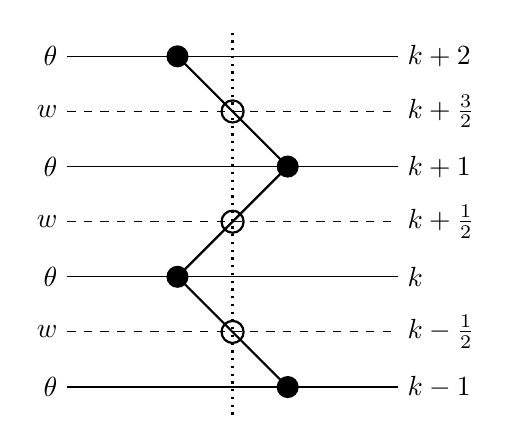
\begin{tikzpicture}[
  scale=0.7,
  cpnt/.style={fill=black}
]
\draw (0,0) -- (6,0) node [at start, anchor=east] {$\theta$} node [at end, anchor=west] {$k-1$};
\draw [dashed] (0,1) -- (6,1) node [at start, anchor=east] {$w$} node [at end, anchor=west] {$k-\frac{1}{2}$};
\draw (0,2) -- (6,2) node [at start, anchor=east] {$\theta$} node [at end, anchor=west] {$k$};
\draw [dashed] (0,3) -- (6,3) node [at start, anchor=east] {$w$} node [at end, anchor=west] {$k+\frac{1}{2}$};
\draw (0,4) -- (6,4) node [at start, anchor=east] {$\theta$} node [at end, anchor=west] {$k+1$};
\draw [dashed] (0,5) -- (6,5) node [at start, anchor=east] {$w$} node [at end, anchor=west] {$k+\frac{3}{2}$};
\draw (0,6) -- (6,6) node [at start, anchor=east] {$\theta$} node [at end, anchor=west] {$k+2$};

\path [cpnt] (4,0) circle [radius=0.2];
\path [cpnt] (2,2) circle [radius=0.2];
\path [cpnt] (4,4) circle [radius=0.2];
\path [cpnt] (2,6) circle [radius=0.2];
\draw [thick] (3,1) circle [radius=0.2];
\draw [thick] (3,3) circle [radius=0.2];
\draw [thick] (3,5) circle [radius=0.2];

\draw [thick] (4,0) -- (2,2) -- (4,4) -- (2,6);
\draw [thick, dotted] (3,-0.5) -- (3,6.5);
\end{tikzpicture}
\end{document}

	\caption{Interpolation of potential temperature on a Lorenz grid.  Solid circles denote values of $\theta$ stored at full levels and the solid line shows the potential temperature profile.  Open circles denote $\theta$ values interpolated onto half levels and the dotted line represents the interpolated profile.  Magnitude of $\theta$ increases to the right.}
	\label{fig:theory:theta-oscillation}
\end{figure}

\section{Gravity waves}
\label{sec:theory:gw}

When an air parcel is forced to rise over a mountain, it experiences a restoring buoyancy force which can create waves that propagate away from the mountain.  These are known as gravity waves, mountain waves, or lee waves.  

Gravity waves play an important role in mesoscale weather.  The waves can trigger convection by propagating through areas of weak stability, they cause clear-air turbulence that affects aircraft \autocite{ray1986}, and can produce very strong downslope winds on the lee slope of the mountain \autocite{holton2003}.

In this section, we briefly present the theory of linear waves and demonstrate their effect on wind and temperature.  In section~\ref{sec:gw}, we relate this theory to the results of a two dimensional experiment in which gravity waves are induced by flow over a wave-shaped mountain range.

Two dimensional waves in the $x-z$ plane are characterised by their frequency, $\omega$, amplitude $\amplitude$, and their horizontal and vertical wavenumbers $k$ and $m$.  In flow over a mountain, the horizontal wavenumber is often related to the spacing between mountain ridges.  By starting with the Boussinesq approximation of the Navier-Stokes equations we can derive the dispersion relation \autocite{lynch-cassano2006}
\begin{align}
	\left( \frac{\partial}{\partial t} + \overline{u} \frac{\partial}{\partial x} \right)^2
	\left( \frac{\partial^2 w'}{\partial x^2} + \frac{\partial^2 w'}{\partial z^2} \right) +
	N^2 \frac{\partial^2 w'}{\partial x^2} = 0
%
	\intertext{where $\overline{u}$ is the mean horizontal wind and $w'$ is the vertical velocity anomaly.  This can be solved by assuming a wave-like solution}
%
	w' = \amplitude \cos \left( kx + mz - \omega t \right) \label{eqn:theory:gw:w-prime}
	\intertext{thus giving the dispersion relation}
	\left( \omega - \overline{u}k \right)^2 
	\left( k^2 + m^2 \right) -
	N^2 k^2 = 0 \label{eqn:theory:gw:dispersion}
\end{align}

The potential temperature anomaly $\theta'$ is a function of background stability $\partial \overline{\theta}/\partial z$ and is \ang{90} out of phase with $w'$, given by \autocite{lynch-cassano2006} \TODO{it'd be nice to derive this from Boussinesq equations but I've struggled to do it myself}
\begin{align}
	\theta' &= \frac{\amplitude}{\omega} \frac{\diff{\overline{\theta}}}{\diff{z}} \sin \phase \label{eqn:theory:gw:theta-prime}
%
	\intertext{where the phase $\phase$ is}
%
	\phase &= kx + mz - \omega t \label{eqn:theory:gw:phase}
\end{align}

\begin{figure}
	\centering
	\documentclass[tikz]{standalone}
\usepackage{bm}
\usetikzlibrary{arrows}
\newcommand{\vect}{\bm}
\newcommand{\del}{\nabla}

\newcommand{\trans}[1]{{#1^\star}}
\newcommand{\surface}{h}
\newcommand{\shellcmd}[1]{\texttt{#1}}
\newcommand{\diffusioncoeff}{\mathcal{D}}
\newcommand{\exner}{\Pi}
\newcommand{\courant}{\mathrm{Co}}

\begin{document}
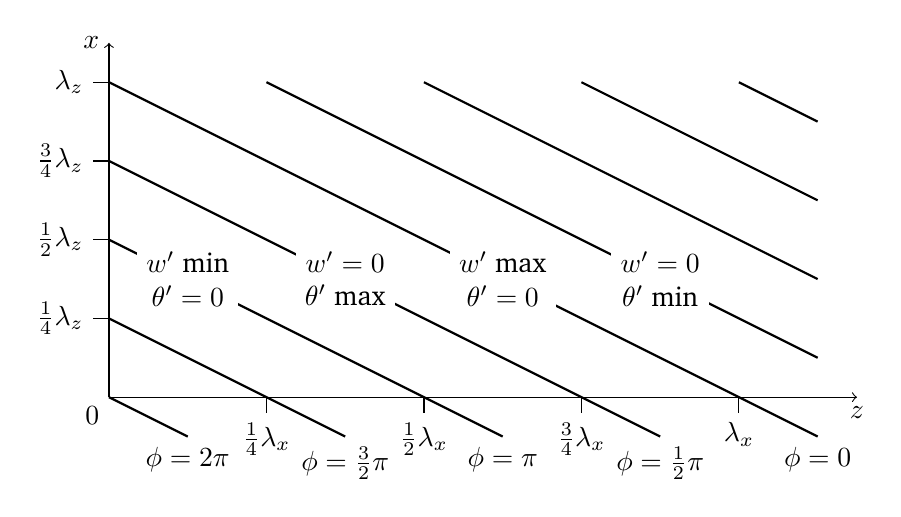
\begin{tikzpicture}[
  cpnt/.style={fill=gray},
  arr/.style={thick, ->},
]
\draw [->] (0,0) -- (0,4.5) node [at end, anchor=east] {$x$} node [at start, anchor=north east] {$0$};
\draw [->] (0,0) -- (9.5,0) node [at end, anchor=north] {$z$};

\draw [thick] (0,0) -- (1,-0.5) node [at end, anchor=north] {$\phi = 2 \pi$};
\draw [thick] (0,1) -- (3,-0.5) node [at end, anchor=north] {$\phi = \frac{3}{2} \pi$};
\draw [thick] (0,2) -- (5,-0.5) node [at end, anchor=north] {$\phi = \pi$};
\draw [thick] (0,3) -- (7,-0.5) node [at end, anchor=north] {$\phi = \frac{1}{2} \pi$};
\draw [thick] (0,4) -- (9,-0.5) node [at end, anchor=north] {$\phi = 0$};
\draw [thick] (2,4) -- (9,0.5);
\draw [thick] (4,4) -- (9,1.5);
\draw [thick] (6,4) -- (9,2.5);
\draw [thick] (8,4) -- (9,3.5);

\node [fill=white, align=center] at (1,1.5) {$w'$ min\\$\theta' = 0$};
\node [fill=white, align=center] at (3,1.5) {$w' = 0$\\$\theta'$ max};
\node [fill=white, align=center] at (5,1.5) {$w'$ max\\$\theta' = 0$};
\node [fill=white, align=center] at (7,1.5) {$w' = 0$\\$\theta'$ min};

\draw (0,1) -- (-0.2,1) node [at end, anchor=east] {$\frac{1}{4} \lambda_z$};
\draw (0,2) -- (-0.2,2) node [at end, anchor=east] {$\frac{1}{2} \lambda_z$};
\draw (0,3) -- (-0.2,3) node [at end, anchor=east] {$\frac{3}{4} \lambda_z$};
\draw (0,4) -- (-0.2,4) node [at end, anchor=east] {$\lambda_z$};

\draw (2,0) -- (2,-0.2) node [at end, anchor=north] {$\frac{1}{4} \lambda_x$};
\draw (4,0) -- (4,-0.2) node [at end, anchor=north] {$\frac{1}{2} \lambda_x$};
\draw (6,0) -- (6,-0.2) node [at end, anchor=north] {$\frac{3}{4} \lambda_x$};
\draw (8,0) -- (8,-0.2) node [at end, anchor=north] {$\lambda_x$};

\end{tikzpicture}
\end{document}

	\caption{Phase relationship between vertical velocity anomalies $w'$ and potential temperature anomalies $\theta'$.  Adapted from \textcite{lynch-cassano2006}.}
	\label{fig:theory:gw:phases}
\end{figure}

Using equations~\ref{eqn:theory:gw:w-prime}, \ref{eqn:theory:gw:theta-prime} and \ref{eqn:theory:gw:phase} we can plot the phase relationships between $w'$ and $\theta'$, shown in figure~\ref{fig:theory:gw:phases}.

Next, we impose a lower boundary condition to simulate flow over an infinite, wave-shaped terrain and find that two types of stationary wave exist.  Consider a surface, the height of which is defined by $h(x)$, such that
\begin{align}
	h(x) &= h_0 \cos \left( kx \right)
%
	\intertext{The flow at any point at the surface must be parallel to that surface (that is, a no normal flow boundary condition)}
%
	w(x,0) &= \frac{\diff{h}}{\diff{t}} \\
	  &= \overline{u} \frac{\partial h}{\partial x} \\
	  &= - \overline{u} k h_0 \sin \left( kx \right) \label{eqn:theory:gw:boundary-cond}
%
	\intertext{Assuming a stationary wave in the form $w'(x, z) = - \overline{u} k h_0 \sin \left( kx + mz \right)$, and noting that $\partial / \partial t = 0$ and $\omega = 0$, we find that the dispersion relation given by equation~\ref{eqn:theory:gw:dispersion} has the solution \autocite{lynch-cassano2006}}
%
	m &= \sqrt{\frac{N^2}{\overline{u}^2} - k^2} \label{eqn:theory:gw:m-dispersion}
\end{align}
which also satisfies the boundary condition given by equation~\ref{eqn:theory:gw:boundary-cond}.  The solution is presented in figure~\ref{fig:theory:gw:propagating} which shows the vertically propagating wave.

We see from equation~\ref{eqn:theory:gw:m-dispersion} that, for $m$ to have a real solution, $|\overline{u}k| < N$.  This constraint cannot be satisfied when the wind is too strong, stability is too weak, or the spacing of mountain ridges is too narrow (that is, $k$ is too large).  In this case, the dispersion relation is instead satisfied by the solution \autocite{lynch-cassano2006}
\begin{align}
	w' &= - \overline{u} k h_0 e^{-mz} \sin \left( kx \right)
\end{align}
As shown in figure~\ref{fig:theory:gw:evanescent}, in this solution, waves decay with height and there is no vertical propagation.  These are often called evanescent waves.

\begin{figure}
	\centering
	\captionsetup[subfigure]{position=b}
	\centering
	\subcaptionbox{Vertically propagating gravity wave \label{fig:theory:gw:propagating}}[0.48\textwidth]{\input{gravityWaves-propagating-plot}}
	\hfill
	\subcaptionbox{Evanescent wave showing rapid decay decay in height and no vertical propagation \label{fig:theory:gw:evanescent}}[0.48\textwidth]{\input{gravityWaves-evanescent-plot}}
%
	\caption{Example vertical cross sections of streamlines for stationary gravity waves over infinite sinusoidal terrain.  Thick dashed lines denote lines of constant phase.  Adapted from \textcite{lynch-cassano2006}.}
	\label{fig:theory:gw:stationary-waves}
\end{figure}


\chapter{Methodology}
\TODO{explain that we're using cartesian coords for everything.  See how Matt Jones justified this.}
\TODO{introduce the equation set and Hilary's discretisation}
\TODO{say something about how OpenFOAM always operates in 3D}

\section{Grid construction}
\label{sec:method:grid}

Two dimensional, regular cartesian grids were created using the OpenFOAM utility, \shellcmd{blockMesh}.  A custom utility was used to modify these orthogonal grids by adjusting the height of points to create terrain following grids.

At the time of writing, OpenFOAM does not directly support cut cell grids\footnote{An enhancement request was filed in 2013 to add support for cartesian cut cells to OpenFOAM, see \url{http://www.openfoam.org/mantisbt/view.php?id=1083}}.  Instead, the \shellcmd{snappyHexMesh} OpenFOAM utility was used to create a grid that approximates the cut cell method.  First, a custom utility was used to move points beneath the surface up to the surface creating small cells near mountain peaks.  Second, a description of the surface was taken from any of the terrain following grids and \shellcmd{snappyHexMesh} was used to intersect the surface with the grid.  The tool removes cells whose centres are below the surface.  An example of the resulting grid is shown in figure~\ref{fig:method:cut-cell}.

The grid is not strictly a cut cell mesh because, when \shellcmd{snappyHexMesh} moves points along the surface according to its heuristics, some points are moved horizontally.  It has not been possible to correct this issue for this project.  This grid is referred to as the `SnapCol' grid throughout this project.

\begin{figure}
	\centerfloat
	\includegraphics[height=2.8in,angle=270]{mesh-snapCol-schaerExp-resting.eps}
	\caption{A `SnapCol' grid created by intersecting the terrain surface with a regular grid as described in section~\ref{sec:method:grid}.  Note that, unlike a true cut cell grid, some small cells have faces at $z = \SI{500}{\meter}$ that are not entirely horizontal.}
	\label{fig:method:cut-cell}
\end{figure}

\section{Discretisation of Euler equations}
\label{sec:method:discretisation}
The fully-compressible Euler equations used in the resting atmosphere test (section~\ref{sec:resting}) and gravity waves test (section~\ref{sec:gw}) are specified as
\begin{align}
& \text{Momentum} & \frac{\partial \rho \vect{u}}{\partial t} + \del \cdot \rho \vect{u} \vect{u} &= \rho \vect{g} - c_p \rho \theta \del \exner \\
%
& \text{Continuity} & \frac{\partial \rho}{\partial t} + \del \cdot \rho \vect{u} &= 0 \\
%
& \text{Potential temperature (flux form)} & \frac{\partial \rho \theta}{\partial t} + \del \cdot \rho \vect{u} \theta &= 0 \\
%
& \text{Potential temperature (advective form)} & \frac{\partial \theta}{\partial t} + \vect{u} \cdot \del \theta &= 0 \\
%
& \text{Equation of state} & \exner^{(1 - \kappa / \kappa)} &= \frac{R \rho \theta}{p_0}
\end{align}
where $\rho$ is the density, $\vect{u}$ is the velocity field, $\vect{g}$ is gravitational acceleration, $c_p$ is the heat capacity of dry air at constant pressure, $\theta$ is the potential temperature, $\exner = \left( p / p_0 \right)^\kappa$ is the Exner function of pressure, $p$ is the pressure, $p_0$ is a reference pressure, $\kappa = R/c_p$, and $R$ is the specific gas constant of dry air.

Here, we outline the placement of prognostic variables, pressure gradient discretisation, and the advection scheme.  Further details of the discretisation are given by \textcite{weller-shahrokhi2014}.

\begin{figure}
	\captionsetup[subfigure]{position=b}
	\centering
	\subcaptionbox{Vertical cross section of geometry}[0.48\textwidth]{\documentclass[tikz]{standalone}
\usepackage{bm}
\newcommand{\vect}{\bm}
\newcommand{\del}{\nabla}

\begin{document}
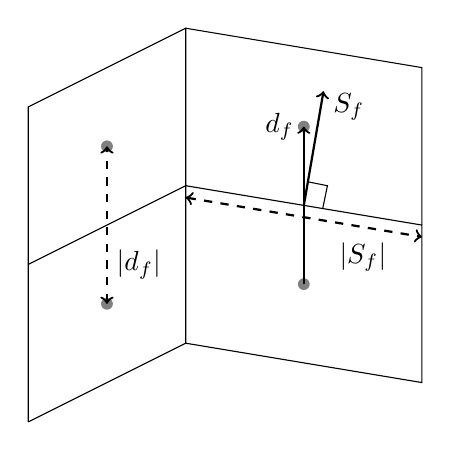
\begin{tikzpicture}[
  scale=0.5,
  cpnt/.style={fill=gray},
  arr/.style={thick, ->},
  mag/.style={dashed, thick, <->}
]
\draw (0,0) --  (4,2)  -- (4,6)  -- (0,4) -- (0,0);
\draw (4,2) --  (10,1) -- (10,5) -- (4,6);
\draw (0,4) --  (0,8)  -- (4,10)  -- (4,6);
\draw (10,5) -- (10,9) -- (4,10);
\path [cpnt] (2,3) circle [radius=0.15];
\path [cpnt] (2,7) circle [radius=0.15];
\path [cpnt] (7,3.5) circle [radius=0.15];
\path [cpnt] (7,7.5) circle [radius=0.15];
\draw [arr] (7,3.5) -- (7,7.5);
\draw [arr] (7,5.5) -- (7.5,8.4);
\node [left] at (7,7.5) {$\vect{d}_f$};
\node [right] at (7.5,8) {$\vect{S}_f$};
\draw [mag] (2,3) -- (2,7);
\node [right] at (2,4) {$|{\vect{d}_f}|$};
\draw [mag] (4,5.7) -- (10,4.7);
\node [below] at (8.5,4.8) {$|{\vect{S}_f}|$};
\draw (7.48,5.42) -- (7.6,6) -- (7.1,6.1);
\end{tikzpicture}
\end{document}
}
	\hfill
	\subcaptionbox{Placement of prognostic variables}[0.48\textwidth]{\documentclass[tikz]{standalone}
\usepackage{bm}
\newcommand{\vect}{\bm}
\newcommand{\del}{\nabla}

\newcommand{\trans}[1]{{#1^\star}}
\newcommand{\surface}{h}
\newcommand{\shellcmd}[1]{\texttt{#1}}
\newcommand{\diffusioncoeff}{\mathcal{D}}
\newcommand{\exner}{\Pi}
\newcommand{\courant}{\mathrm{Co}}

\begin{document}
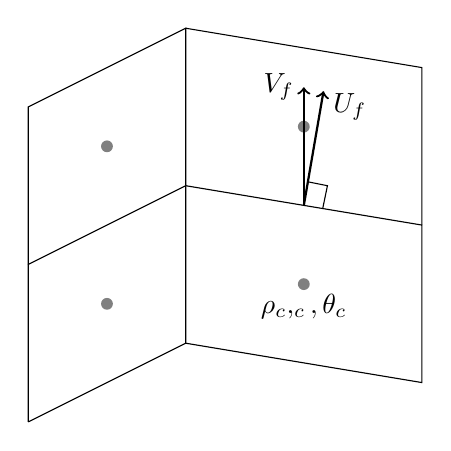
\begin{tikzpicture}[
  scale=0.5,
  cpnt/.style={fill=gray},
  arr/.style={thick, ->},
  mag/.style={dashed, thick, <->}
]
\draw (0,0) --  (4,2)  -- (4,6)  -- (0,4) -- (0,0);
\draw (4,2) --  (10,1) -- (10,5) -- (4,6);
\draw (0,4) --  (0,8)  -- (4,10)  -- (4,6);
\draw (10,5) -- (10,9) -- (4,10);
\path [cpnt] (2,3) circle [radius=0.15];
\path [cpnt] (2,7) circle [radius=0.15];
\path [cpnt] (7,3.5) circle [radius=0.15];
\path [cpnt] (7,7.5) circle [radius=0.15];
\draw [arr] (7,5.5) -- (7,8.5);
\draw [arr] (7,5.5) -- (7.5,8.4);
\node [below] at (7,3.5) {$\rho_c, \exner_c, \theta_c$};
\node [left] at (7,8.5) {$V_f$};
\node [right] at (7.5,8) {$U_f$};
\draw (7.48,5.42) -- (7.6,6) -- (7.1,6.1);
\end{tikzpicture}
\end{document}
}
	\caption{Geometric placement of prognostic variables in two dimensions.  Adapted from \textcite{weller-shahrokhi2014}.}
	\label{fig:method:placement}
\end{figure}

\TODO{pressure gradient}

\TODO{cubic upwind advection scheme}

\section{Energy measures}
\label{sec:method:energy}

Energy conservation is desirable in the discretisation of the Euler equations.  In the resting atmosphere test detailed in section~\ref{sec:resting}, energy is conserved in the analytic solution, but not in all numerical approximations.  The normalised energy change $\Delta E$ at time $t$ is found by comparing with the initial energy measure, hence
\begin{align}
	\Delta E(t) &= \frac{E(t) - E(t = \SI{0}{\second})}{E(t = \SI{0}{\second})}
\end{align}
Three energy measures are considered, where the volume integral of some field $\varphi$ is the volume-weighted sum given by
\begin{align}
	\int_V \varphi \diff{V} &= \frac{\sum_c \varphi_c V_c}{\sum_c V_c}
\end{align}
First, kinetic energy $E_K$ is calculated as \TODOcite
\begin{align}
	E_K(t) &= \int_V \frac{1}{4} \sum_{f \in \: c} \frac{\vect{u} \cdot \vect{S}_f \: \vect{u} \cdot \vect{d}_f}{V_c} \diff{V}
%
	\intertext{where \TODO{define variables if needed}  Second, potential energy $E_P$ is}
%
	E_P(t) &= - \int_V \rho \vect{g} \cdot \vect{x_c} \diff{V}
%
	\intertext{where $\vect{x}_c$ is the position vector of the centre of cell $c$.  Third, the internal energy $E_I$ is \TODOcite}
%
	E_I(t) &= \int_V \rho \theta \Pi c_v \diff{V}
\end{align}
where \TODO{define variables if needed}

\chapter{Results}
Three test cases were performed over idealised terrain in two dimensions.  First, we report on the numerical errors associated with the horizontal advection of a scalar tracer.  Second, spurious flow and energy conservation are examined for a stable atmosphere initially at rest.  Third, \TODO{gravity waves...}  For each test, results on BTF, SLEVE and the cut cell style `SnapCol' grid are compared.  \TODO{any more?}

\section{Horizontal tracer advection}
\label{sec:advection}

Following \textcite{schaer2002}, a tracer is transported above orography by solving the advection equation for a prescribed horizontal wind.  This challenges the accuracy of the advection scheme in the presence of grid distortions.
The wind profile, terrain profile and initial tracer field are shown in Figure~\ref{fig:advection:initial}.

\subsection{Specification}
The domain is \SI{300}{\kilo\meter} wide and \SI{25}{\kilo\meter} high.  The terrain is wave-shaped, specified by the surface height $\surface$ such that
\begin{subequations}
\label{eqn:advection:schaerCos}
\begin{align}
	\surface(x) &= \cos^2 \left( \frac{\pi x}{\lambda} \right) \surface^\star
%
	\intertext{where}
%
	\surface^\star(x) &= \left\{ \begin{array}{l l}
		h_0 \cos^2 \left( \frac{\pi x}{2a} \right) & \quad \text{if $| x | < a$} \\
		0 & \quad \text{otherwise}
	\end{array} \right.
\end{align}
\end{subequations}
where $a = \SI{25}{\kilo\meter}$ is the mountain half-width, $h_0 = \SI{3}{\kilo\meter}$ is the maximum mountain height, and $\lambda = \SI{8}{\kilo\meter}$ is the wavelength.  On the SLEVE grid, the large-scale component $\surface_1$, as described in section~\ref{sec:theory:tf}, is given by
\begin{align}
	\surface_1(x) &= \frac{1}{2}\surface^\star(x)
\end{align}
and $s_1 = \SI{15}{\kilo\meter}$ is the large scale height, and $s_2 = \SI{2.5}{\kilo\meter}$ is the small scale height.  The optimisation of SLEVE by \textcite{leuenberger2010} is not used, so the exponent $n = 1$.
For comparison, the same tests were performed with no orography, such that $\surface = \SI{0}{\kilo\meter}$ everywhere.

The wind is entirely horizontal and is prescribed as
\begin{align}
	u(z) = u_0 \left\{ \begin{array}{l l}
		1 & \quad \text{if $z \geq z_2$} \\
		\sin^2 \left( \frac{\pi}{2} \frac{z - z_1}{z_2 - z_1} \right) & \quad \text{if $z_1 < z < z_2$} \\
		0 & \quad \text{otherwise}
	\end{array} \right.	
\end{align}
where $u_0 = \SI{10}{\meter\per\second}$, $z_1 = \SI{4}{\kilo\meter}$ and $z_2 = \SI{5}{\kilo\meter}$.
This results in a constant wind aloft, and zero flow at \SI{4}{\kilo\meter} and below.
A tracer $\varphi$ is positioned upstream above the height of the terrain.  It has the shape
\begin{align}
	\varphi(x, z) &= \varphi_0 \left\{ \begin{array}{l l}
		\cos^2 \left( \frac{\pi r}{2} \right) & \quad \text{if $r \leq 1$} \\
		0 & \quad \text{otherwise}
	\end{array} \right.
%
\intertext{having radius $r$ given by}
%
	r &= \sqrt{
		\left( \frac{x - x_0}{A_x} \right)^2 + 
		\left( \frac{z - z_0}{A_z} \right)^2
	}
\end{align}
where $A_x = \SI{25}{\kilo\meter}$, $A_z = \SI{3}{\kilo\meter}$ are the horizontal and vertical half-widths respectively, and $\varphi_0 = 1$ is the maximum magnitude of the anomaly.  At $t = \SI{0}{\second}$, the anomaly is centred at $(x_0, z_0) = (\SI{-50}{\kilo\meter}, \SI{9}{\kilo\meter})$ so that the anomaly is upwind of the mountain and well above the maximum terrain height of \SI{3}{\kilo\meter}.  Analytic solutions can be found by adjusting the anomaly centre such that $x_0 = ut$.

\begin{figure}
	\centerfloat
	\input{advection-initial-plot}
	\caption{Vertical cross section of the two-dimensional advection test showing the horizontal wind profile, surface terrain profile and tracer field at $t = \SI{0}{\second}$ on a $\SI{300}{\kilo\meter} \times \SI{25}{\kilo\meter}$ domain.  Adapted from \textcite{schaer2002}.}
	\label{fig:advection:initial}
\end{figure}

\subsection{Discretisation}
The OpenFOAM solver \shellcmd{scalarTransportFoam} was used to implicitly solve the advection equation in flux form
\begin{align}
	\frac{\partial \varphi}{\partial t} + \del \cdot \left( \vect{u} \varphi \right) = 0 \label{eq:advection:continuous}
\end{align}
The solver uses a velocity field with values defined at cell centres, and linearly interpolates onto cell faces during the model initialisation phase.

The time derivative is solved implicitly using a backward-in-time, second order accurate scheme defined as \autocite{openfoam-progguide}.  At time level $n$, the time derivative, $\partial \varphi / \partial t$, is
\begin{align}
	\frac{\partial}{\partial t} \int_V \varphi \diff V = \frac{
		3 \left( \varphi V \right)^{(n)} - 
		4 \left( \varphi V \right)^{(n-1)} + 
		\left( \varphi V \right)^{(n-2)}
	}{2 \Delta t}
\end{align}

Spatial discretisation follows the finite volume method described in section~\ref{sec:theory:fv}, using the upwind-biased advection scheme described in section~\ref{sec:method:discretisation}.
The domain is discretised onto a grid having $300 \times 50$ cells such that $\Delta x = \SI{1}{\kilo\meter}$ and $\Delta \trans{z} = \SI{500}{\meter}$.  Unlike \textcite{schaer2002} who use periodic lateral boundaries, we use a fixed value of 0 at the inlet boundary and zero gradient boundaries elsewhere.
Tests are integrated forward in time for \SI{10000}{\second} with a timestep $\Delta t = \SI{25}{\second}$.

\subsection{Diagnostics}
Results of advection are evaluated in four ways.  First, tracer contours are plotted to visualise the extent to which tracer shape and magnitude are preserved.  Second, tracer error contours are found by subtracting the analytic solution from the numerical solution.  Both sets of contours enable results to be compared with those from \textcite{schaer2002}.  Third, preservation of tracer magnitude is quantified by finding the minimum and maximum tracer values at the end of the simulation.

Finally, error norms are calculated at $t = \SI{10000}{\second}$ by comparing with the analytic solution.  The $\ell^2$ error norm is defined as
\begin{align}
\ell^2 = \sqrt{\frac{\sum \left( \varphi - \varphi_T \right)^2 V}{\sum V}}
\end{align}
where $\varphi$ is the numerical tracer value, $\varphi_T$ is the analytic value and $V$ is the cell volume.  Because the test is two dimensional, the cell volume is equivalent to the cell area.  

\subsection{Analysis}
\begin{figure}
	\captionsetup[subfigure]{position=b}
	\centering
	\subcaptionbox{BTF (negative contours at $t = \SI{10000}{\second}$ near mountain peak shown as dashed red lines) \label{fig:advection:cubicUpwind:btf}}[0.49\textwidth]{\input{advection-btf-schaerCos-cubicUpwindCPCFit-contour-plot}}
	\hfill
	\subcaptionbox{BTF from \textcite{schaer2002} (negative contours shown as dashed lines) \label{fig:advection:schaer:btf}}[0.49\textwidth]{\vspace{0.43in}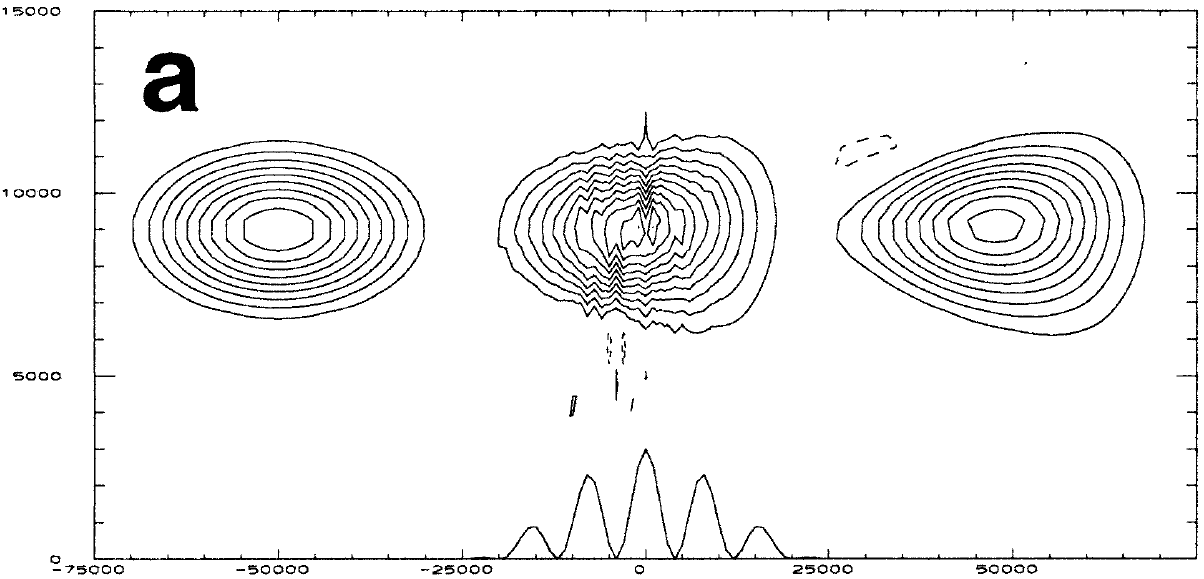
\includegraphics[height=1.2in]{img/schaer-btf-centred.png}}
\\
	\subcaptionbox{SLEVE \label{fig:advection:cubicUpwind:sleve}}[0.49\textwidth]{\input{advection-sleve-schaerCos-cubicUpwindCPCFit-contour-plot}}
	\hfill
	\subcaptionbox{SLEVE from \textcite{schaer2002} \label{fig:advection:schaer:sleve}}[0.49\textwidth]{\vspace{0.43in}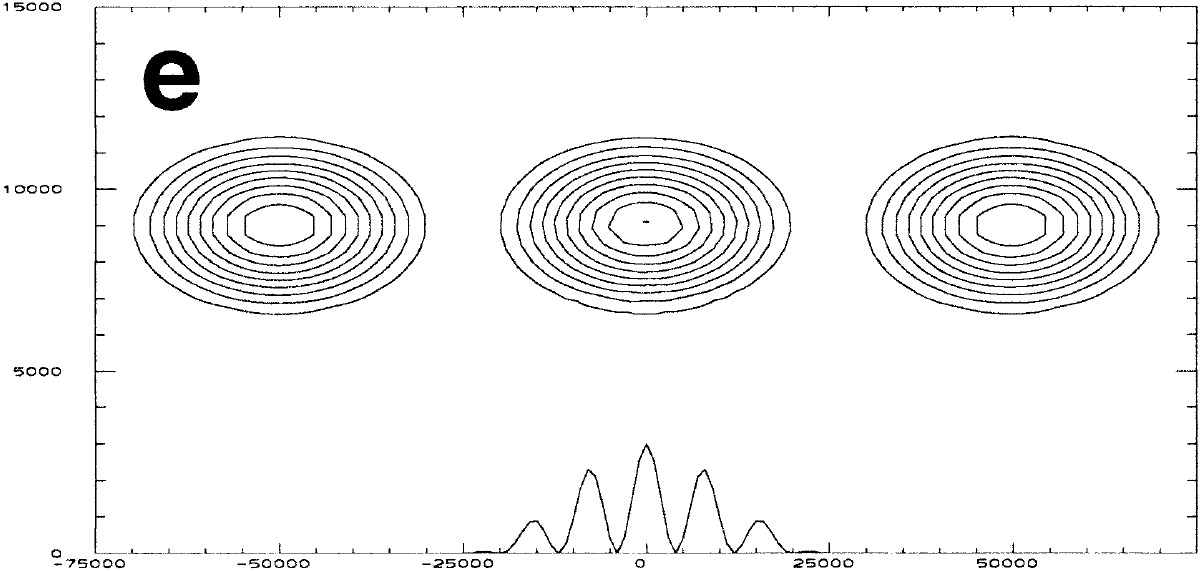
\includegraphics[height=1.2in]{img/schaer-sleve-centred.png}}
\\
	\subcaptionbox{SnapCol grid \label{fig:advection:cubicUpwind:snapCol}}[0.49\textwidth]{\input{advection-snapCol-schaerCos-cubicUpwindCPCFit-contour-plot}}
	\hfill
	\subcaptionbox{Analytic solution on a regular grid \label{fig:advection:analytic}}[0.49\textwidth]{\input{advection-noOrography-analytic-contour-plot}}
%
	\caption{Horizontally advected tracer contours at $t = \SI{0}{\second}$, \SI{5000}{\second} and \SI{10000}{\second}.  Figures (\protect\subref{fig:advection:cubicUpwind:btf}), (\protect\subref{fig:advection:cubicUpwind:sleve}), and (\protect\subref{fig:advection:cubicUpwind:snapCol}) use the upwind-biased scheme described in section~\ref{sec:method:discretisation}.  Figures (\protect\subref{fig:advection:schaer:btf}) and (\protect\subref{fig:advection:schaer:sleve}) show the results of the second-order centred difference scheme from \textcite{schaer2002}.  Contour intervals are every 0.1.}
	\label{fig:advection:cubicUpwind}
\end{figure}

\begin{figure}
	\captionsetup[subfigure]{position=b}
	\centering
	\subcaptionbox{BTF \label{fig:advection:error:btf:cubicUpwind}}[0.49\textwidth]{\includegraphics[width=1.3in,angle=270]{openfoam/cases/advection/btf/schaerCos/cubicUpwindCPCFit/10000/tracer-contour-error.eps}}
	\hfill
	\subcaptionbox{BTF from \textcite{schaer2002} \label{fig:advection:error:schaer:btf}}[0.49\textwidth]{\vspace{0.1in}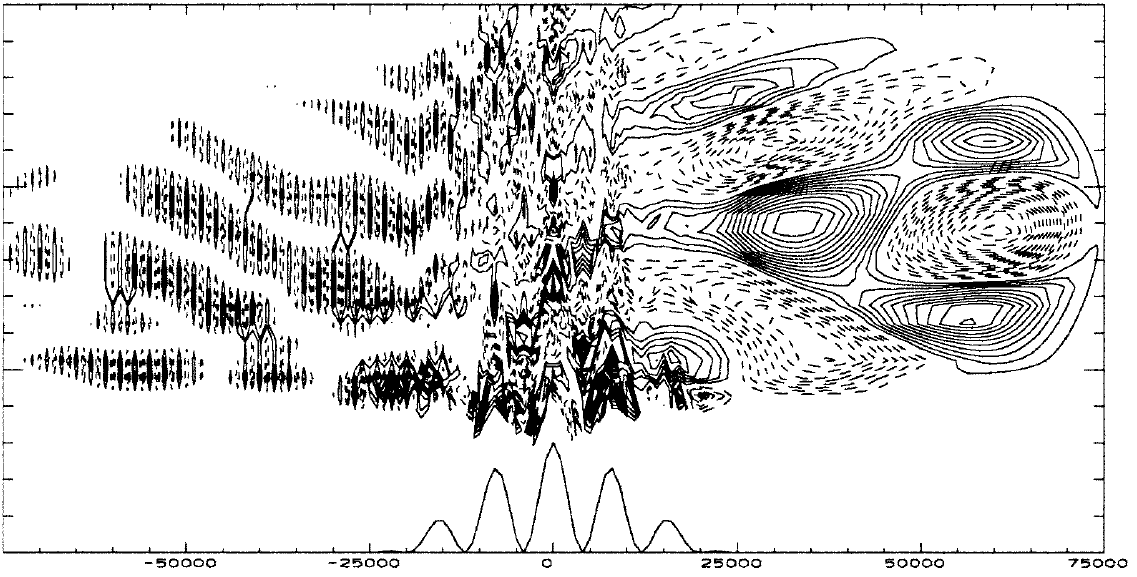
\includegraphics[height=1.2in]{img/schaer-btf-centred-error.png}} \\
%
	\subcaptionbox{SLEVE \label{fig:advection:error:sleve:cubicUpwind}}[0.49\textwidth]{\includegraphics[width=1.3in,angle=270]{openfoam/cases/advection/sleve/schaerCos/cubicUpwindCPCFit/10000/tracer-contour-error.eps}}
	\hfill
	\subcaptionbox{SLEVE from \textcite{schaer2002} \label{fig:advection:error:schaer:sleve}}[0.49\textwidth]{\vspace{0.1in}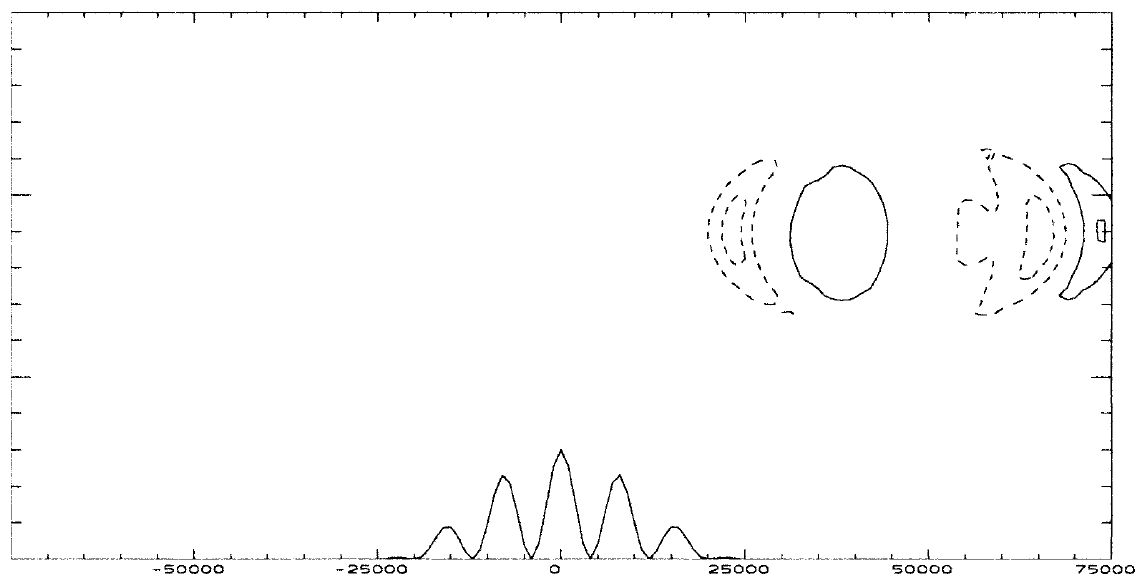
\includegraphics[height=1.2in]{img/schaer-sleve-centred-error.png}} \\
%
	\subcaptionbox{Regular grid \label{fig:advection:error:noOrography:cubicUpwind}}[0.49\textwidth]{\includegraphics[width=1.3in,angle=270]{openfoam/cases/advection/noOrography/cubicUpwindCPCFit/10000/tracer-contour-error.eps}}
	\hfill
	\subcaptionbox{Regular grid from \textcite{schaer2002} \label{fig:advection:error:schaer:noOrography}}[0.49\textwidth]{\vspace{0.1in}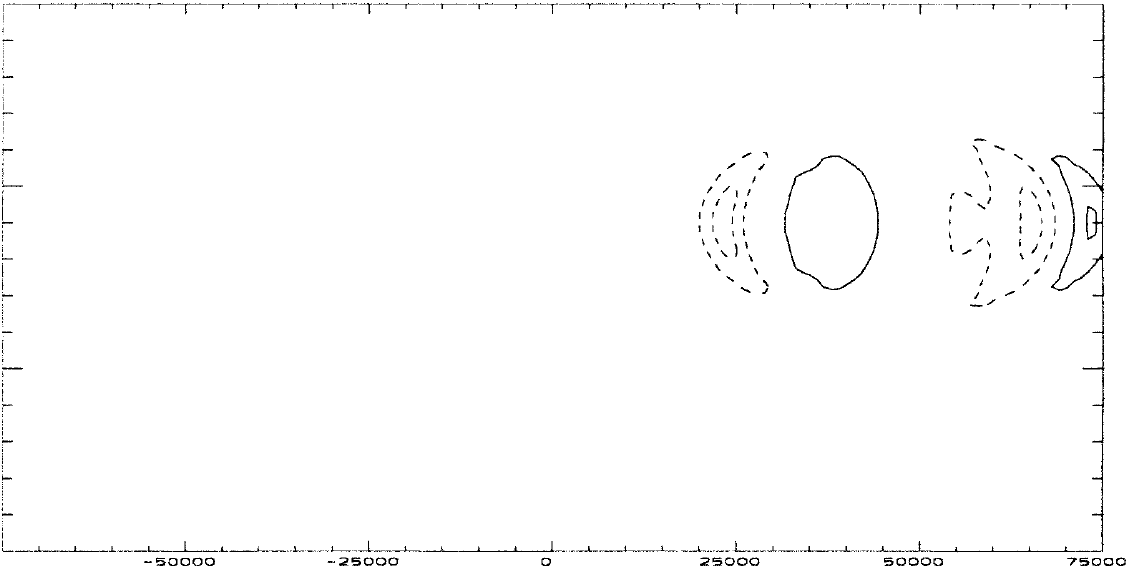
\includegraphics[height=1.2in]{img/schaer-noOrography-centred-error.png}} \\
%
	\caption{Errors in horizontal tracer advection at $t = \SI{10000}{\second}$.  Figures (\protect\subref{fig:advection:error:btf:cubicUpwind}), (\protect\subref{fig:advection:error:sleve:cubicUpwind}) and (\protect\subref{fig:advection:error:noOrography:cubicUpwind}) use the upwind-biased scheme.  Figures (\protect\subref{fig:advection:error:schaer:btf}), (\protect\subref{fig:advection:error:schaer:sleve}) and (\protect\subref{fig:advection:error:schaer:noOrography}) show the error of the second-order centred difference scheme from \textcite{schaer2002}.  Contour intervals are every 0.01, with negative contours denoted by dashed lines.}
	\label{fig:advection:error}
\end{figure}

Results of advection are presented in figure~\ref{fig:advection:cubicUpwind}.
On the BTF grid, the tracer suffers from distortion over the mountain and some artefacts just above the mountain remain as the tracer moves over it.  Comparing figures~\ref{fig:advection:cubicUpwind:btf} and \ref{fig:advection:schaer:btf}, we see that the tracer retains its shape far better than the result from \textcite{schaer2002} that uses a second-order centred difference scheme.  This is expected since the upwind-biased cubic scheme has a larger stencil and higher order accuracy.  Comparing figures~\ref{fig:advection:error:btf:cubicUpwind} and \ref{fig:advection:error:schaer:btf} we see that, unlike the results from \textcite{schaer2002}, errors on the BTF grid are confined to regions around the tracer and near the mountain peak.

As seen in figure~\ref{fig:advection:cubicUpwind:sleve}, results on the SLEVE grid are much closer to the analytic solution on a regular grid (figure~\ref{fig:advection:analytic}).  The tracer retains its shape throughout the simulation and does not suffer from any noticeable distortion.  We find that accuracy is slightly better than the result from \textcite{schaer2002} (see figures~\ref{fig:advection:error:sleve:cubicUpwind} and \ref{fig:advection:error:schaer:sleve}).  Unlike \textcite{schaer2002}, a further improvement in accuracy is seen on a regular grid, as shown in figure~\ref{fig:advection:error:noOrography:cubicUpwind}.

Since the SnapCol grid is entirely regular away from the surface, it is unsurprising that the results (shown in figure~\ref{fig:advection:cubicUpwind:snapCol}) are the same as advection on a regular grid (not shown).  This result agrees with that found by \textcite{good2013}.

At $t = \SI{0}{\second}$, the tracer ranges between zero and one.  Over time, new extrema are generated because the upwind-biased advection scheme is not monotonic.  This is most evident on the BTF grid where the stationary artefacts above the mountain peak reach a minimum of \input{openfoam/cases/advection/btf/schaerCos/cubicUpwindCPCFit/min.txt} by the end of the simulation.  The results of the second-order centred difference scheme of \textcite{schaer2002} show significant negative tracer values as evidenced by the dashed contours in figure~\ref{fig:advection:schaer:btf}.  Minimum values remain close to zero on the SLEVE, SnapCol and regular grids.  All grids show some decrease in maximum tracer magnitude and, once again, the decrease is most severe on the BTF grid.  Results of tracer extrema on all grids are compared to the analytic solution in figure~\ref{fig:wobblyTracerAdvection:ranges:horizontal} and the values are given in table~\ref{tab:advection:errors} on page~\pageref{tab:advection:errors}.

Because the upwind-biased advection scheme is not monotonic, one source of new extrema is a divergent velocity field.  Areas of convergence will increase tracer magnitude and areas of divergence will reduce it.  Although the continuous velocity field in this test is non-divergent, this is not necessarily true of the discrete velocity field, especially where the grid is non-orthogonal.

\begin{figure}
	\centering
	\documentclass[tikz]{standalone}
\usepackage{bm}
\input{mathmacros}
\begin{document}
\begin{tikzpicture}[
  scale=0.75,
  cpnt/.style={fill=gray},
  vertex/.style={fill=black},
  arr/.style={ultra thick, ->},
  mag/.style={dashed, thick, <->}
]
\draw (0,0) -- (4,0);
\draw (0,3) -- (4,3);
\draw [dashed, thick] (0,0) -- (0,3);
\draw [dashed, thick] (4,0) -- (4,3);
\draw (4,3) -- (8,5) -- (8,2) -- (4,0);
\draw (0,0) -- (-4,-3) -- (-4,0) -- (0,3);
\path [cpnt] (-2,0) circle [radius=0.15] node [above right] {$c_0$};
\path [cpnt] (2,1.5) circle [radius=0.15] node [above right] {$c_1$};
\path [cpnt] (6,2.5) circle [radius=0.15] node [above right] {$c_2$};

\draw (0,1.5) circle [radius=0.15];
\draw (4,1.5) circle [radius=0.15];o

\draw [thick, ->] (-0.5,1.5) -- (0.5,1.5) node [above] {$f_\mathrm{in}$};
\draw [ultra thick, ->] (3,1.5) -- (5,1.5) node [above] {$f_\mathrm{out}$};
\end{tikzpicture}
\end{document}

	\caption{Flux through two faces, shown with dashed lines, in a rectangular cell in the region of vertical wind shear.  Because the surrounding cells are non-orthogonal, interpolation onto cell faces results in a net outward flux which leads to a decrease in tracer magnitude.  Cell centres are denoted by grey circles, face centres are denoted by open circles.}
	\label{fig:advection:flux}
\end{figure}

Let us consider the fluxes in and out of the vertically-oriented faces, $\fin$ and $\fout$, of a rectangular cell in the region of vertical wind shear such that its cell centre $c_1$ has a height $\SI{4}{\kilo\meter} < z < \SI{5}{\kilo\meter}$.  To its left is a cell whose centre, $c_0$, is lower and to its right, a cell whose centre, $c_2$, is higher.  This situation is shown in figure~\ref{fig:advection:flux}.

During model initialisation, the solver interpolates velocities at cell centres onto cell faces, such that $\fin$ is interpolated from $c_0$ and $c_1$, and $\fout$ is an interpolation of $c_1$ and $c_2$.  Remember that horizontal wind is increasing with height, $u(c_2) > u(c_1) > u(c_0)$, and so $\fout > \fin$.  Therefore, there is a net divergence in the rectangular cell, which leads to a decrease in tracer magnitude.

\begin{figure}
	\captionsetup[subfigure]{position=b}
	\centering
	\subcaptionbox{BTF \label{fig:advection:div:btf}}[0.49\textwidth]{\includegraphics[width=1.8in,angle=270]{openfoam/cases/advection/btf/schaerCos/cubicUpwindCPCFit/0/divU.eps}}
	\hfill
	\subcaptionbox{SLEVE \label{fig:advection:div:sleve}}[0.49\textwidth]{\includegraphics[width=1.8in,angle=270]{openfoam/cases/advection/sleve/schaerCos/cubicUpwindCPCFit/0/divU.eps}}
%
	\includegraphics[height=5in,angle=270]{legends/divU.eps}
%
	\caption{\TODO{divergence. don't forget units}}
	\label{fig:advection:div}
\end{figure}

\TODO{now we can talk about how we measured divergence, and the results we got, and what we can conclude from this}

The $\ell^2$ error norms are also summarised in table~\ref{tab:advection:errors}.  Errors on the BTF grid are an order of magnitude greater than the three other grids tested.  The cut cell grid offers only a small error reduction compared to the SLEVE grid.  Even on the BTF grid, the upwind-biased advection scheme is far more tolerant of grid distortions than results of the fourth-order centred scheme from \textcite{schaer2002} (not shown).



\section{Resting atmosphere}
\label{sec:resting}

This two-dimensional test simulates a stably stratified atmosphere in hydrostatic balance.  Since there are no net forces, the analytical solution should remain at rest.  The test specification follows that from \textcite{klemp2011}, and challenges the accuracy of the calculation of the horizontal pressure gradient.  An inversion layer causes nonlinear processes that further tax the model \autocite{good2013}.

\subsection{Specification}
Following \textcite{weller-shahrokhi2014}, the domain is \SI{20}{\kilo\meter} wide and \SI{20}{\kilo\meter} high, which is narrower than \textcite{klemp2011} in order to reduce simulation time.  The wave-shaped mountain profile is taken from \textcite{schaer2002} where the surface height $h$ is given by
\begin{align}
	\surface(x) = \surface_0 \exp \left( - \left( \frac{x}{a} \right)^2 \right) \cos^2 \left( \frac{\pi x}{\lambda} \right) \label{eqn:resting:mountain}
\end{align}
where $a = \SI{5}{\kilo\meter}$ is the mountain half-width, $h_0 = \SI{1}{\kilo\meter}$ is the maximum mountain height and $\lambda = \SI{4}{\kilo\meter}$ is the wavelength.  For the optimised SLEVE grid, the large-scale component $\surface_1$, described in section~\ref{sec:theory:tf}, is specified as
\begin{align}
\surface_1(x) = \frac{1}{2} \surface_0 \exp \left( - \left( \frac{x}{a} \right)^2 \right)
\end{align}
and, following \cite{leuenberger2010}, $s_1 = \SI{4}{\kilo\meter}$ is the large scale height, $s_2 = \SI{1}{\kilo\meter}$ is the small scale height, and the optimal exponent value of $n = 1.35$ is used.  Results are compared with the numerical solution with no orography.

The initial thermodynamic conditions have a surface temperature of $\theta_0 = \SI{288}{\kelvin}$ and constant stability with Brunt-V\"ais\"al\"a frequency $N = \SI{0.01}{\per\second}$ everywhere, except for a more stable layer of $N = \SI{0.02}{\per\second}$ between $\SI{2}{\kilo\meter} \leq z \leq \SI{3}{\kilo\meter}$.

\subsection{Diagnostics}
Two metrics were used to measure the model error.  First, maximum vertical velocity is measured at each timestep.  An analytic solution has no vertical velocity $w$ since the atmosphere is at rest.  However, numerical error in calculating the horizontal pressure gradient give rise to spurious vertical velocities which become more severe over steep terrain \autocite{klemp2011}.

Second, normalised energy change $\Delta E$ is measured for each timestep as described in section~\ref{sec:method:energy}.  The total normalised energy change is the sum of normalised kinetic, potential, and internal energy changes.
An analytic solution would conserve total energy such that $\Delta E(t) = 0\;\forall\;t$.  As discussed in \textcite{weller-shahrokhi2014}, energy is not exactly conserved in the model presented because of damping by the advection scheme and inexact transfer between kinetic, internal and potential energy.

\subsection{Discretisation}
The simulation uses the discretisation of the fully-compressible Euler equations described in section~\ref{sec:method:discretisation}.  The domain is discretised on a grid having $40 \times 40$ cells such that $\Delta x = \Delta z = \SI{0.5}{\kilo\meter}$.  All boundary conditions are no normal flow.  The simulation is integrated forward by 5 hours with a timestep $\Delta t = \SI{100}{\second}$.  Unlike \textcite{klemp2011}, there is no eddy diffusion in the equation set.

\subsection{Results}
\begin{figure}
	\captionsetup[subfigure]{position=b}
	\centering
	\subcaptionbox{Model results \label{fig:resting:w:model}}[0.58\textwidth]{\input{resting-w-plot}}
	\hfill
	\subcaptionbox{Results from \textcite{klemp2011}}[0.4\textwidth]{\vspace{0.27in}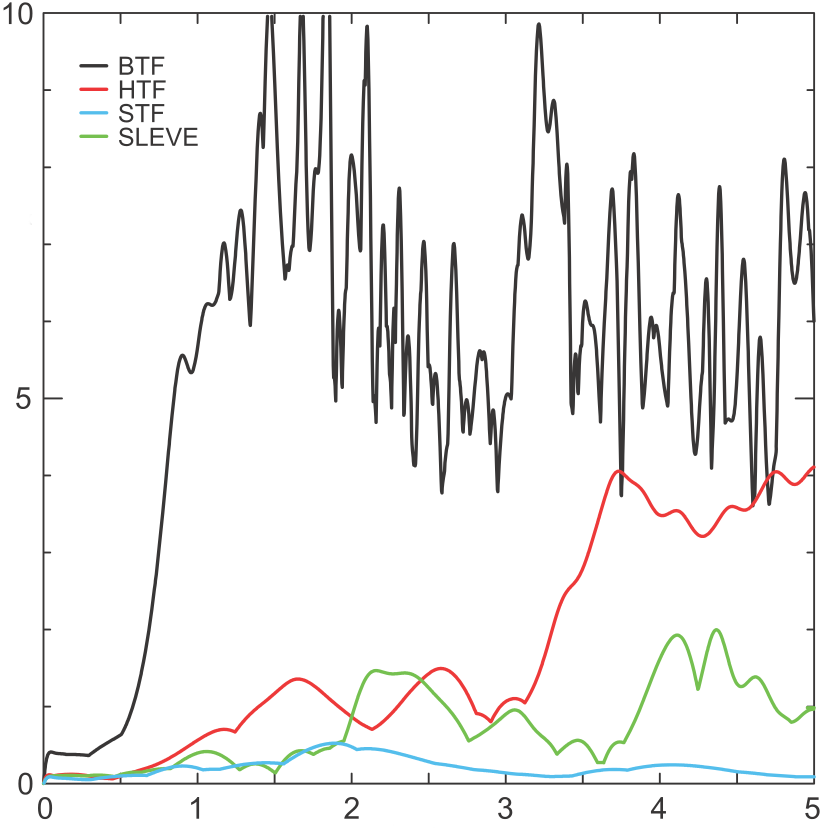
\includegraphics[height=2in]{img/klemp-w.png}}
	\caption{Maximum spurious vertical velocity $w$ in the resting atmosphere test compared with results from \textcite{klemp2011}.  Note that vertical scales differ.}
	\label{fig:resting:w}
\end{figure}

Test results for BTF, optimised SLEVE, and SnapCol grids are compared with results on a regular grid with no orography.  On the BTF grid, spurious vertical velocity $w$ reaches $\sim \SI{0.35}{\meter\per\second}$, which is significantly less than the velocities of $\sim \SI{10}{\meter\per\second}$ found by \textcite{klemp2011} (see figure~\ref{fig:resting:w}, note different vertical scales).  An oscillation develops after 4 hours, the cause of which is not yet known.  Unlike the results from \textcite{klemp2011}, the optimised SLEVE grid does not significantly reduce $w$ compared to BTF.  Since the model and its initialisation are the same, results on the BTF and optimised SLEVE grids are also in agreement with \textcite{weller-shahrokhi2014}.

The SnapCol grid results in a significantly smaller maximum vertical velocity of less than \SI{1e-3}{\meter\per\second}.  The smallest error of $\sim \SI{1e-10}{\meter\per\second}$ is found on the regular grid.  This error may be due to loss of precision when OpenFOAM loads the initial conditions, which are in discrete hydrostatic balance, but the source of the error is not certain.

\begin{figure}
	\captionsetup[subfigure]{position=b}
	\centering
	\subcaptionbox{Cell centres at centre of uncut cells leading to some cell centres below the ground \label{fig:resting:good:uncut}}[0.49\textwidth]{\input{resting-good-uncut-plot}}
	\hfill
	\subcaptionbox{Cell centres at centre of cut cells \label{fig:resting:good:cut}}[0.49\textwidth]{\input{resting-good-cut-plot}}
%
	\caption{Placement of cell centres on a two-dimensional cut cell grid.  The model from \textcite{good2013} has some cell centres below the ground (B. Good 2014, personal communication).  The arrows denote an estimated horizontal gradient between two adjacent cells of a scalar value stored at cell centres.}
	\label{fig:resting:good}
\end{figure}

Using a timestep of \SI{1.01}{\second}, \textcite{good2013} found the maximum vertical velocity in their cut cell model was \SI{1e-12}{\meter\per\second}, which is better than any result from the experiments in this project.  However, in that model, cell centres are in the centre of the uncut cell, resulting in the centre of some cut cells being below the ground, as shown in figure~\ref{fig:resting:good} (B. Good 2014, personal communication).  This means that the grid is effectively regular when calculating horizontal and vertical gradients.

\begin{figure}
	\captionsetup[subfigure]{position=b}
	\centering
	\subcaptionbox{Total normalised energy changes on terrain following grids \label{fig:resting:energy:total-tf}}[0.32\textwidth]{\input{resting-energy-total-tf-plot}}
	\hfill
	\subcaptionbox{As (\subcaptionref{fig:resting:energy:total-tf}), but on the SnapCol grid \label{fig:resting:energy:total-snapCol}}[0.32\textwidth]{\input{resting-energy-total-snapCol-plot}}
	\hfill
	\subcaptionbox{As (\subcaptionref{fig:resting:energy:total-tf}), but on a regular grid with no orography \label{fig:resting:energy:total-noOrography}}[0.32\textwidth]{\input{resting-energy-total-noOrography-plot}}
	\\
	\subcaptionbox{Kinetic ($E_K$), potential ($E_P$) and internal ($E_I$) normalised energy changes on BTF grid \label{fig:resting:energy:btf}}[0.32\textwidth]{\input{resting-energy-btf-plot}}
	\hfill
	\subcaptionbox{As (\subcaptionref{fig:resting:energy:btf}), but on the optimised SLEVE grid \label{fig:resting:energy:sleve}}[0.32\textwidth]{\input{resting-energy-sleve-plot}}
	\hfill
	\subcaptionbox{As (\subcaptionref{fig:resting:energy:btf}), but on the SnapCol grid.  Note the different vertical scale from figures~(\subcaptionref{fig:resting:energy:btf}) and (\subcaptionref{fig:resting:energy:sleve}). \label{fig:resting:energy:snapCol}}[0.32\textwidth]{\input{resting-energy-snapCol-plot}}
	\caption{Comparison of normalised energy changes on BTF, optimised SLEVE and SnapCol grids for the resting atmosphere test.}
	\label{fig:resting:energy}
\end{figure}

Examining normalised energy change, shown in figure~\ref{fig:resting:energy:total-tf}, we find that there is a net loss of energy on BTF and optimised SLEVE grids.  However, there is a period of energy gain on the optimised SLEVE grid during the first two hours, and an upward trend in energy after 3 hours on the BTF grid.  The cause of the energy gain is the subject of further work (see chapter~\ref{sec:further-work}).

Energy is better conserved on the SnapCol grid, the energy loss being more than two orders of magnitude smaller than the terrain following grids (figure~\ref{fig:resting:energy:total-snapCol}).  This compares favourably with the best possible energy conservation for this model as found on a regular grid (figure~\ref{fig:resting:energy:total-noOrography}).

The spurious motion generated by horizontal pressure gradient errors leads to a positive change in kinetic energy, evident in figures~\ref{fig:resting:energy:btf} and~\ref{fig:resting:energy:sleve}.  Compared to both terrain following grids, internal and potential energy conservation is three orders of magnitude better on the SnapCol grid (\ref{fig:resting:energy:snapCol}).  As noted by \textcite{weller-shahrokhi2014}, the model converts between potential and internal energy on timescales of less than an hour.  This can be seen by the mirroring between $E_P$ and $E_I$ plots, and we confirm that this local energy conservation property is present in all three grids (figures~\ref{fig:resting:energy:btf}, \subcaptionref{fig:resting:energy:sleve} and \subcaptionref{fig:resting:energy:snapCol}).

\TODO{if I want to compare to Zaengl (and also Good), I would need to try the same experiment with 4km high mountain, too}

\TODO{I could compare theta field (as done by Klemp)}


\section{Gravity waves}
\label{sec:gw}

Following \textcite{schaer2002}, uniform flow over an idealised two-dimensional mountain ridge induces gravity waves in a stable atmosphere.  As described in section~\ref{sec:theory:gw}, large-scale waves propagate away from the surface and small-scale evanescent waves decay rapidly above the terrain.

\subsection{Specification}
Following \textcite{melvin2010}, the domain is \SI{300}{\kilo\meter} wide and \SI{30}{\kilo\meter} high.  The mountain profile has the same form as equation~\ref{eqn:resting:mountain} but with a lower maximum height of $\surface_0 = \SI{250}{\meter}$.  As in the resting atmosphere test, $a = \SI{5}{\kilo\meter}$ is the mountain half-width and $\lambda = \SI{4}{\kilo\meter}$ is the wavelength.  On the optimised SLEVE grid, $s_1 = \SI{5}{\kilo\meter}$ is the large scale height, $s_2 = \SI{2}{\kilo\meter}$ is the small scale height and the optimal exponent value $n = 1.35$ as in the previous test.

The initial thermodynamic conditions have a surface temperature of $\theta_0 = \SI{288}{\kelvin}$ and constant stability with $N = \SI{0.01}{\per\second}$ everywhere.  A constant horizontal wind $u = \SI{10}{\meter\per\second}$ is prescribed at the inlet boundary.

\subsection{Discretisation}
The test uses the discretisation of the Euler equations described in section~\ref{sec:method:discretisation}.  The domain is discretised on a grid having $600 \times 100$ cells such that $\Delta x = \SI{0.5}{\kilo\meter}$ and $\Delta z = \SI{300}{\meter}$.  Sponge layers are added to the upper \SI{10}{\kilo\meter} and leftmost \SI{10}{\kilo\meter} at the inlet boundary to damp the reflection of waves.
The term $\mu \rho \vect{u}$ is subtracted from the momentum equation (equation~\ref{eqn:method:momentum}) where the damping function $\mu$ is adapted from \textcite{melvin2010} such that
\begin{align}
	\mu(x, z) &= \mu_\mathrm{upper} + \mu_\mathrm{inlet} \\
	\mu_\mathrm{upper}(z) &= \begin{cases}
		\overline{\mu} \sin^2 \left( \frac{\pi}{2} \frac{z - z_B}{H - z_B} \right) & \text{if } z \geq z_B \\
		0 & \text{otherwise} \\
	\end{cases} \\
	\mu_\mathrm{inlet}(x) &= \begin{cases}
		\overline{\mu} \sin^2 \left( \frac{\pi}{2} \frac{x_I - x}{x_I - x_0} \right) & \text{if } x < x_I \\
		0 & \text{otherwise}
	\end{cases}
\end{align}
where $\overline{\mu} = 1.2$ is the damping coefficient, $z_B = \SI{20}{\kilo\meter}$ is the bottom of the sponge layer, $H = \SI{30}{\kilo\meter}$ is the top of the domain, $x_0 = \SI{-150}{\kilo\meter}$ is the leftmost limit of the domain and $x_I = \SI{-140}{\kilo\meter}$ is the rightmost extent of the inlet sponge layer.  The sponge layer is only active on faces whose normal is vertical so that it damps vertical momentum only.

Note that, while the domain itself is \SI{30}{\kilo\meter} in height, for the purposes of generating of BTF and SLEVE grids, the domain height is set to \SI{20}{\kilo\meter} because the sponge layer occupies the uppermost \SI{10}{\kilo\meter}.

No slip conditions are imposed on the top and bottom boundaries and the outlet is zero gradient.  For Exner, hydrostatic balance is prescribed on all boundaries.  Following \textcite{melvin2010}, the simulation is integrated forward by 5 hours with a timestep $\Delta t = \SI{8}{\second}$.

\subsection{Analysis}

\begin{figure}
	\centering
	\begin{subfigure}[b]{0.48\textwidth}
		\includegraphics[height=2.6in,angle=270]{data/gravityWaves-btf-schaerExp-h/18000/w.eps}\vspace{2em}
		\caption{BTF}
		\label{fig:gw:w:btf}
	\end{subfigure}
	\hfill
	\begin{subfigure}[b]{0.48\textwidth}
		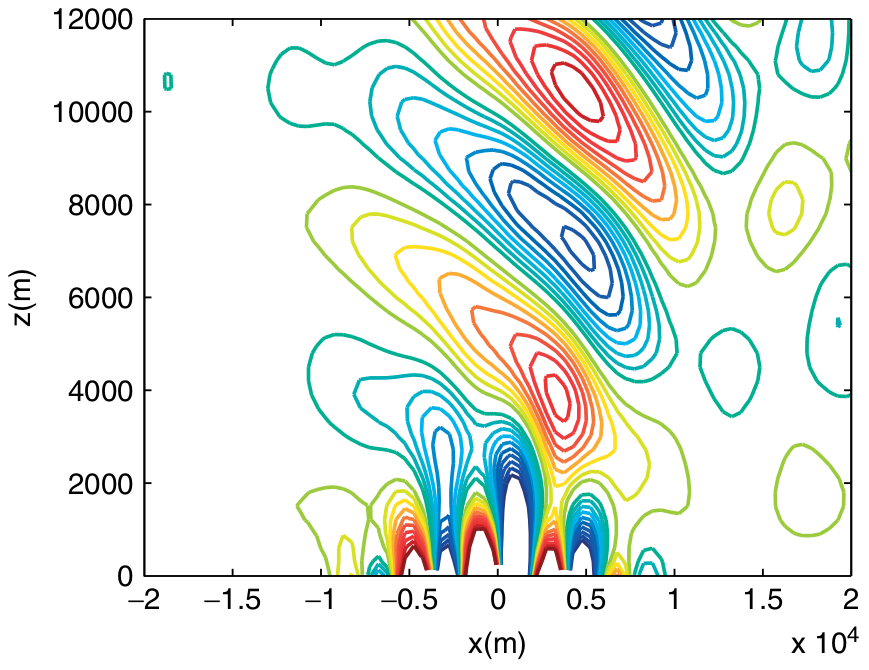
\includegraphics[height=2in]{img/melvin-7a.png}
		\caption{Mass-conserving semi-implicit semi-Lagrangian solution from \textcite{melvin2010}}
		\label{fig:gw:w:melvin}
	\end{subfigure} \\
%
	\begin{subfigure}[b]{0.48\textwidth}
		\includegraphics[height=2.6in,angle=270]{data/gravityWaves-sleve-schaerExp-h/18000/w.eps}
		\caption{SLEVE}
		\label{fig:gw:w:sleve}
	\end{subfigure}
	\hfill
	\begin{subfigure}[b]{0.48\textwidth}
		\includegraphics[height=2.6in,angle=270]{data/gravityWaves-sleve-schaerExp-h/18000/thetaDiff.eps}
		\caption{SLEVE}
		\label{fig:gw:thetaDiff:sleve}
	\end{subfigure} \\
%
	\begin{subfigure}[b]{0.48\textwidth}
		\includegraphics[height=2.6in,angle=270]{data/gravityWaves-sleve-schaerExp-h/18000/w.eps}\vspace{3em}
		\caption{SnapCol}
		\label{fig:gw:w:snapCol}
	\end{subfigure}
	\hfill
	\begin{subfigure}[b]{0.48\textwidth}
		\shortstack[c]{\includegraphics[height=2.6in,angle=270]{data/gravityWaves-snapCol-schaerExp-h/18000/thetaDiff.eps} \\
			\smallskip \hspace{1em} \includegraphics[height=2.4in,angle=270]{legends/thetaDiff.eps}}
		\caption{SnapCol}
		\label{fig:gw:thetaDiff:snapCol}
	\end{subfigure}
%
	\caption{Vertical cross section of vertical velocity contours (\subcaptionref{fig:gw:w:btf}, \subcaptionref{fig:gw:w:sleve} and \subcaptionref{fig:gw:w:snapCol}) and potential temperature anomalies in Kelvin (\subcaptionref{fig:gw:thetaDiff:sleve} and \subcaptionref{fig:gw:thetaDiff:snapCol}) from the gravity waves test after 5 hours.  Vertical velocity contours are every \SI{5e-2}{\meter\per\second} with solid lines denoting ascent and dashed lines descent.}
	\label{fig:gw:w}
\end{figure}

Comparing vertical velocity contours between BTF and SLEVE show few visible differences (figures~\ref{fig:gw:w:btf}, \subcaptionref{fig:gw:w:sleve}).  Evanescent waves are visible as dense contours immediately above the mountain ridges and the large-scale hydrostatic waves propagate vertically.  We verify the two wave types using the linear theory discussed in section~\ref{sec:theory:gw}.  The horizontal wavelength between each mountain peak is specified as $\lambda = \SI{4e3}{\meter}$, so $k = 2 \pi / \lambda \approx \SI{1.57e-3}{\per\meter}$.  The condition for evanescent waves is that $| \overline{u}k | \geq N$.  Since this test specifies $N = \SI{0.01}{\per\second}$ and $\overline{u} = \SI{10}{\meter\per\second}$, we find that the condition is satisfied.

The mountain half-width is specified to be $a = \SI{5e3}{\meter}$, so the large-scale wavelength is \SI{1e4}{\meter} and the horizontal wavenumber $k \approx \SI{6.28e-4}{\per\meter}$.  In this case, $| \overline{u}k | < N$, so waves propagate vertically.  Hence, we have shown that both propagating and evanescent waves are generated by this particular configuration of stability, wind speed, and mountain profile.

Since the same model was used, vertical velocities match those from \textcite{weller-shahrokhi2014}.  Vertical velocities on the SnapCol grid are similar to the terrain following results (figure~\ref{fig:gw:w:snapCol}).  All three results are in agreement with a semi-implicit, semi-Lagrangian simulation from \textcite{melvin2010} (see figure~\ref{fig:gw:w:melvin}).

\begin{figure}
	\captionsetup[subfigure]{position=b}
	\centering
	\subcaptionbox{BTF (gravity waves test) \label{fig:gw:flow:btf}}[0.49\textwidth]{\includegraphics[width=1.5in,angle=270]{data/gravityWaves-btf-schaerExp-h/18000/UfZoom.eps}}
	\subcaptionbox{SnapCol (gravity waves test) \label{fig:gw:flow:snapCol}}[0.49\textwidth]{\includegraphics[width=1.5in,angle=270]{data/gravityWaves-snapCol-schaerExp-h/18000/UfZoom.eps}} \\
%
	\subcaptionbox{BTF (thermal advection test) \label{fig:wobblyThetaAdvection:flow:btf}}[0.49\textwidth]{\includegraphics[width=1.5in,angle=270]{openfoam/cases/wobblyThetaAdvection/btf/schaerExp/cubicUpwindCPCFit/0/Uzoom.eps}}
	\subcaptionbox{SnapCol (thermal advection test) \label{fig:wobblyThetaAdvection:flow:snapCol}}[0.49\textwidth]{\includegraphics[width=1.5in,angle=270]{openfoam/cases/wobblyThetaAdvection/snapCol/schaerExp/cubicUpwindCPCFit/0/Uzoom.eps}} \\
%
	\caption{Vertical cross section of velocity vectors in the centremost \SI{10}{\kilo\meter} and lowest \SI{1.2}{\kilo\meter}.  In the gravity waves test, the velocity field after 5 hours follows the terrain and is qualitatively similar on (\subcaptionref{fig:gw:flow:btf}) the BTF grid, (\subcaptionref{fig:gw:flow:snapCol}) the SnapCol grid, and the SLEVE grid (not shown).  For the thermal advection test described in section~\ref{sec:wobblyThetaAdvection}, the terrain following velocity field is prescribed.  It is designed to imitate the velocity field of the gravity waves test, and is shown here on the BTF grid (\subcaptionref{fig:wobblyThetaAdvection:flow:btf}) and SnapCol grid (\subcaptionref{fig:wobblyThetaAdvection:flow:snapCol}).}
	\label{fig:gw:flow}
\end{figure}

Examining the velocity vector field we find that the flow is qualitatively similar between the BTF grid (figure~\ref{fig:gw:flow:btf}), SnapCol grid (figure~\ref{fig:gw:flow:snapCol}), and SLEVE grid (not shown).  Flow near the ground follows the terrain, accelerating as it passes over the mountain peaks, with velocities becoming more horizontal aloft.  

\begin{figure}
	\captionsetup[subfigure]{position=b}
	\centering
	%
	\subcaptionbox{BTF $h_0 = \SI{250}{\meter}$ \label{fig:gw:div:btf}}[0.49\textwidth]{\includegraphics[width=1.8in,angle=270]{data/gravityWaves-btf-schaerExp-h/18000/divUf.eps}}
	\hfill
	\subcaptionbox{BTF $h_0 = \SI{500}{\meter}$ \label{fig:gw:div:btf-dh}}[0.49\textwidth]{\includegraphics[width=1.8in,angle=270]{data/gravityWaves-btf-schaerExp-doubleHigh-h/18000/divUf.eps}} \\
%
	\subcaptionbox{SLEVE $h_0 = \SI{250}{\meter}$ \label{fig:gw:div:sleve}}[0.49\textwidth]{\includegraphics[width=1.8in,angle=270]{data/gravityWaves-sleve-schaerExp-h/18000/divUf.eps}}
	\hfill
	\subcaptionbox{SLEVE $h_0 = \SI{500}{\meter}$ \label{fig:gw:div:sleve-dh}}[0.49\textwidth]{\includegraphics[width=1.8in,angle=270]{data/gravityWaves-sleve-schaerExp-doubleHigh-h/18000/divUf.eps}} \\
%
	\subcaptionbox{SnapCol $h_0 = \SI{250}{\meter}$ \label{fig:gw:div:snapCol}}[0.49\textwidth]{\includegraphics[width=1.8in,angle=270]{data/gravityWaves-snapCol-schaerExp-h/18000/divUf.eps}}
	\hfill
	\subcaptionbox{SnapCol $h_0 = \SI{500}{\meter}$ \label{fig:gw:div:snapCol-dh}}[0.49\textwidth]{\includegraphics[width=1.8in,angle=270]{data/gravityWaves-snapCol-schaerExp-doubleHigh-h/18000/divUf.eps}} \\
%
	\includegraphics[height=5in,angle=270]{legends/divU.eps}
%
	\caption{Divergence (\si{\per\second}) of the discrete velocity field in the centremost \SI{20}{\kilo\meter} and lowest \SI{8}{\kilo\meter} for a mountain height of $h_0 = \SI{250}{\meter}$ on the BTF grid (\subcaptionref{fig:gw:div:btf}), SLEVE grid (\subcaptionref{fig:gw:div:sleve}), and SnapCol grid (\subcaptionref{fig:gw:div:snapCol}), and for a mountain height of $h_ = \SI{500}{\meter}$ on the BTF, SLEVE and SnapCol grids (\subcaptionref{fig:gw:div:btf-dh}, \subcaptionref{fig:gw:div:sleve-dh} and \subcaptionref{fig:gw:div:snapCol-dh} respectively).}
	\label{fig:gw:div}
\end{figure}

As shown in figure~\ref{fig:gw:div:btf}, \ref{fig:gw:div:sleve} and \ref{fig:gw:div:snapCol}, divergence in the velocity field was found to be negligible everywhere except the lowest layer on all grids.  Magnitude of divergence is slightly greater on the SnapCol grid.

\begin{figure}
	\captionsetup[subfigure]{position=b}
	\centering
	\subcaptionbox{SLEVE $\surface_0 = \SI{250}{\meter}$ \label{fig:gw:thetaDiffZoom:sleve}}[\textwidth]{\includegraphics[width=1.4in,angle=270]{data/gravityWaves-sleve-schaerExp-h/18000/nonlinearMomentumZoom.eps}} \\
	\subcaptionbox{SnapCol $\surface_0 = \SI{250}{\meter}$ \label{fig:gw:thetaDiffZoom:snapCol}}[\textwidth]{\includegraphics[width=1.4in,angle=270]{data/gravityWaves-snapCol-schaerExp-h/18000/nonlinearMomentumZoom.eps}} \\
	\subcaptionbox{SLEVE $\surface_0 = \SI{500}{\meter}$ \label{fig:gw:thetaDiffZoom:sleve-dh}}[\textwidth]{\includegraphics[width=1.4in,angle=270]{data/gravityWaves-sleve-schaerExp-doubleHigh-h/18000/nonlinearMomentumZoom.eps}} \\
	\subcaptionbox{SnapCol $\surface_0 = \SI{500}{\meter}$ \label{fig:gw:thetaDiffZoom:snapCol-dh}}[\textwidth]{\includegraphics[width=1.4in,angle=270]{data/gravityWaves-snapCol-schaerExp-doubleHigh-h/18000/nonlinearMomentumZoom.eps}} \\
%
	\includegraphics[height=5in,angle=270]{legends/nonlinearMomentumZoom_thetaDiff.eps}
	\caption{Vertical cross section of potential temperature anomalies (\si{\kelvin}) in the centermost \SI{10}{\kilo\meter} and lowest \SI{1.2}{\kilo\meter} after 5 hours.  Subfigures (\subcaptionref{fig:gw:thetaDiffZoom:sleve}) and (\subcaptionref{fig:gw:thetaDiffZoom:snapCol}) show close up views of the potential temperature anomalies in figures~\ref{fig:gw:thetaDiff:sleve} and \ref{fig:gw:thetaDiff:snapCol} respectively.  Note the different colour scale from figure~\ref{fig:gw:w}.}
	\label{fig:gw:thetaDiffZoom}
\end{figure}

Potential temperature anomalies are similar on all grids, having a similar shape to vertical velocity contours (SLEVE grid figure~\ref{fig:gw:thetaDiff:sleve}, SnapCol grid figure~\ref{fig:gw:thetaDiff:snapCol}, BTF grid not shown).  As predicted by the gravity wave theory discussed in section~\ref{sec:theory:gw}, potential temperature and vertical velocity anomalies are out of phase by \ang{90}.

Examining more closely the potential temperature anomaly on the SnapCol grid, in the lee of the mountain the bottommost layer is anomalously warm and the layer above it is anomalously cold (figure~\ref{fig:gw:thetaDiffZoom:snapCol}).  Potential temperature increases with height because the simulated atmosphere is stable, so these anomalies serve to reduce the stability near the ground.  The anomalies are not sufficiently large to destabilise the atmosphere, however.   Therefore, vertical motion is not expected, and was not observed, near the ground on the lee side.   Whilst turbulent motion does cause thermal mixing in the real atmosphere, there is no viscosity in the model equations, so the thermal anomalies should not be present.  The feature is not present on the SLEVE grid (figure~\ref{fig:gw:thetaDiffZoom:sleve}) or BTF grid (not shown).

Figure~\ref{fig:gw:exner-theta} plots vertical profiles of Exner and potential temperature in the lowest \SI{1}{\kilo\meter} in the lee of the mountain at $x = \SI{50}{\kilo\meter}$.  The Exner function decreases linearly and is identical on BTF and SnapCol grids.  The potential temperature profile is linear on the BTF grid but a slight zig-zag is present on the SnapCol grid in the lowest two layers, corresponding to the warm and cold anomalies.  This profile shares the same shape as the example presented in figure~\ref{fig:theory:theta-oscillation}.
This implies that the computational mode of the Lorenz vertical staggering has been excited, because the zig-zag is present in the potential temperature profile, but not in the Exner profile.

Another test was performed in which the mountain height was doubled such that $\surface_0 = \SI{500}{\meter}$, with all other parameter values unchanged.  Divergence of the velocity field was visually unchanged on the BTF grid (figure~\ref{fig:gw:div:btf-dh}), but magnitude of divergence increased above the mountain peaks on the SLEVE and SnapCol grids (figures~\ref{fig:gw:div:sleve-dh} and \ref{fig:gw:div:snapCol-dh} respectively).

Overall potential temperature anomalies increase in magnitude because the gravity wave amplitude is larger, but these waves do not reach all the way to the ground.  In the lowest two layers, results on the SLEVE grid are similar for both mountain heights (see figures~\ref{fig:gw:thetaDiffZoom:sleve} and \ref{fig:gw:thetaDiffZoom:sleve-dh}).  On the SnapCol grid, the Lorenz computational mode is more severe.  Figure~\ref{fig:gw:exner-theta} also shows that potential temperature errors are no longer confined to the lowest two layers, but extend beyond \SI{1200}{\meter} above the ground.  Differences in potential temperature from the initial profile are summarised in table~\ref{tab:theta-sample}.

In section~\ref{sec:wobblyTracerAdvection}, we found that errors were largest when advecting a tracer over the SnapCol grid in a terrain following velocity field.  This suggests that the computational mode is excited by errors in the upwind-biased advection scheme.  A further experiment is presented in section~\ref{sec:wobblyThetaAdvection} to test this hypothesis.

\begin{figure}
	\captionsetup[subfigure]{position=b}
	\centering
	\subcaptionbox{Vertical profiles of the Exner function of pressure, $\exner$, and potential temperature, $\theta$, in the gravity waves experiment.  Exner profile is visually identical on all grids for both $\surface_0 = \SI{250}{\meter}$ and $\surface_0 = \SI{500}{\meter}$; for clarity, Exner profile is only plotted for the SLEVE grid.  The computational mode is manifested as a zig-zag in potential temperature on the SnapCol grid.  The double height mountain increases the severity of the computational mode, but has negligible effect on the SLEVE grid (not shown).  All results on the BTF grid are qualitatively the same as those on the SLEVE grid (not shown). \label{fig:gw:exner-theta}}[\textwidth]{\input{gravityWaves-schaerExp-h-exnerTheta-plot}} \\
%
	\subcaptionbox{Vertical potential temperature profile from the test of terrain following advection of a stable thermal profile, described in section~\ref{sec:wobblyThetaAdvection}.  Results on the BTF grid are visually identical to the initial potential temperature profile (not shown).  \label{fig:wobblyThetaAdvection:theta}}[\textwidth]{\input{wobblyThetaAdvection-schaerExp-theta-plot}}
%
	\caption{Vertical profiles in the lowest \SI{1}{\kilo\meter} in the lee of the mountain at $x = \SI{50}{\kilo\meter}$ after 5 hours.}
	\label{fig:exner-theta}
\end{figure}

\begin{table}
\centering
\begin{tabular}{ r @{\hspace{2em}} S[table-format=1.3] S[table-format=1.3] S[table-format=1.3] S[table-format=1.3] S[table-format=1.3] S[table-format=1.3] S[table-format=1.3] S[table-format=1.3]}
\toprule
			& \multicolumn{3}{c}{Gravity waves, $h_0 = \SI{250}{\meter}$}	& \multicolumn{3}{c}{Gravity waves, $h_0 = \SI{500}{\meter}$}	& \multicolumn{2}{c}{Thermal advection} \\
Height (\si{\meter})	& {BTF}	& {SLEVE}	&	{SnapCol}	& {BTF}	& {SLEVE}	& {SnapCol} & {BTF} & {SnapCol} \\ \midrule
150 & -0.003 & -0.001 & 0.046 & -0.003 & 0.031 & 0.254 & -0.001 & -0.643 \\
450 & 0.006  & 0.013 & -0.05 & 0.006 & 0.012 & -0.169 & 0.002 & 0.652 \\
750 & 0.032  & 0.03 & 0.023 & 0.032 & 0.055 & -0.169 & -0.003 & -0.033 \\
1050 & 0.046 & 0.04 & 0.041 & 0.046 & 0.106 & 0.069 & 0.004 & -0.031 \\
\bottomrule
\end{tabular}
%
\caption{Difference in potential temperature (\si{\kelvin}) from the initial profile in the lowest \SI{1200}{\meter} at $x = \SI{50}{\kilo\meter}$ for the gravity waves test (section~\ref{sec:gw}) and thermal advection test (section~\ref{sec:wobblyThetaAdvection}).}
\label{tab:theta-sample}
\end{table}

\begin{figure}
	\captionsetup[subfigure]{position=b}
	\centering
	\subcaptionbox{Maximum Courant number \label{fig:gw:courant:max}}[0.49\textwidth]{\input{gravityWaves-courant-max-plot}}
	\hfill
	\subcaptionbox{Mean Courant number \label{fig:gw:courant:mean}}[0.49\textwidth]{\input{gravityWaves-courant-mean-plot}}
	%
	\caption{Courant numbers on BTF, SLEVE and SnapCol grids for the gravity waves test.}
	\label{fig:gw:courant}
\end{figure}

Little evidence of the `small cell' problem associated with cut cell grids, discussed in section~\ref{sec:theory:shaving}, was found on the SnapCol grid.  At each timestep, the maximum and mean Courant number for all cells in the grid was calculated.  Whilst initially larger on the SnapCol grid, the maximum Courant number eventually converges for all three grids (figure~\ref{fig:gw:courant:max}).  After 5 hours, the maximum Courant number gradually rises (not shown).  In figure~\ref{fig:gw:courant:mean}, we see that the mean Courant number is similar across all grids, but also increases slowly throughout the simulation.  It is likely that this is because the gravity waves are still amplifying, leading to a steady increase in wind speeds.

\begin{figure}
	\centering
	\documentclass[tikz]{standalone}
\usepackage{bm}
\usetikzlibrary{arrows}
\input{mathmacros}
\input{dissertationmacros}
\begin{document}
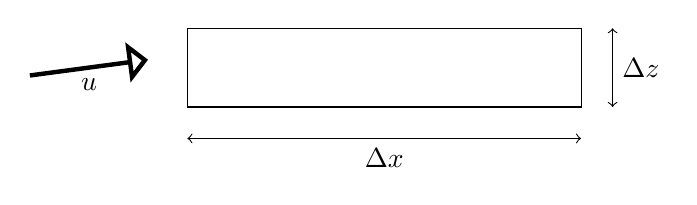
\begin{tikzpicture}[
  cpnt/.style={fill=gray},
  arr/.style={thick, ->},
]
\draw (5,1) rectangle (10,2);

\draw [<->] (5,0.6) -- (10,0.6) node [midway, below] {$\Delta x$};
\draw [<->] (10.4,1) -- (10.4,2) node [midway, right] {$\Delta z$};

\draw [->, >=open triangle 90, ultra thick] (3,1.4) -- (4.5,1.6) node [midway, below] {$\vect{u}$};
\end{tikzpicture}
\end{document}

	\caption{Nearly-horizontal flow through a thin, rectangular cell in the $x-z$ plane.  Because the vertical velocity component is small, the cell height $\Delta z$ has a negligible effect on the two-dimensional Courant number.}
	\label{fig:gw:small-cell}
\end{figure}

The lack of evidence for the small cell problem be explained by considering flow through a two-dimensional, rectangular cell in the $x-z$ plane in which $\Delta x$ is several times larger than $\Delta z$ (figure~\ref{fig:gw:small-cell}).  Using equation~\ref{eqn:method:courant} and assuming a uniform flow $\vect{u} = ( u, 0, w )^\intercal$, the Courant number is
\begin{align}
	\courant &= \frac{\Delta t}{\Delta x \Delta z} \left( u \Delta z + w \Delta x \right)
%
	\intertext{When the flow is almost horizontal, $u \gg w$, so}
%
	\courant &\approx \frac{u \Delta t}{\Delta x}
\end{align}
That is, the two-dimensional Courant number reduces to the one-dimensional Courant number.  Hence, the cell height $\Delta z$ has little effect on the CFL criterion.

In the gravity waves test, vertical motion is induced by the terrain and, for the shallow gradients used in this test, horizontal velocities dominate.

In conclusion, test results were similar on all grids and vertical velocities are in good agreement with results from the literature.  On the SnapCol grid, thin cells had little effect on the timestep because the flow was predominantely horizontal.  Errors in potential temperature were found near the ground in the lee of the mountain on the SnapCol grid and these were attributed to the Lorenz computational mode.  It is possible that regions of relatively large divergence and convergence immediately above the ground are a cause of these thermal errors.

\section{Terrain following tracer advection}
\label{sec:wobblyTracerAdvection}

In the horizontal advection test, results were more accurate when the flow was aligned with grid layers: on the cut cell grid results were accurate, but distortions in the BTF grid led to increased error.  This terrain following advection test is designed to determine the nature of these errors by prescribing a velocity field that is aligned with the layers of the BTF grid.  If errors are caused by skewness or grid non-uniformity (described in section~\ref{sec:theory:skewness}), we expect least accuracy on terrain following grids since they are less orthogonal.  However, if errors are caused by flow crossing grid layers, then results are expected to be less accurate on the SnapCol grid.

\subsection{Specification}
The spatial domain, mountain profile, initial tracer profile and discretisation are the same as those in the horizontal tracer advection test (section~\ref{sec:advection}).  The velocity field, however, is defined using a streamfunction $\Psi$ so that the velocity field is non-divergent.  Unlike the horizontal advection test, flow extends from the top of the domain all the way to the ground.  It is defined so that flow is everywhere tangential to BTF coordinate surfaces given by equation~\ref{eqn:theory:btf} such that
\begin{align}
	\Psi(x,z) &= H \frac{z - h}{H - h}
%
	\intertext{The horizontal and vertical components of velocity, $u$ and $w$ are then given by}
%
	u &= \frac{\partial \Psi}{\partial z} \quad,\quad  w = -\frac{\partial \Psi}{\partial x}
%
	\intertext{Hence, for the mountain profile given in equation~\ref{eqn:advection:schaerCos} we find}
%
	u &= \frac{H}{H - h} \quad,\quad w = H \frac{\partial h}{\partial x} \frac{H - z}{\left( H - h \right)^2} \label{eqn:wobblyTracerAdvection:velocity} \\
	\frac{\partial h}{\partial x} &= - h_0 \pi \left[ 
		\frac{1}{\lambda} \cos^2 \left( \frac{\pi x}{2a} \right) \sin \left( \frac{2 \pi x}{\lambda} \right) +
		\frac{1}{2a} \cos^2 \left( \frac{\pi x}{\lambda} \right) \sin \left( \frac{\pi x}{a} \right)
	\right]
\end{align}
The resulting velocity field is shown in figure~\ref{fig:wobblyTracer:u}.

\begin{figure}
	\centering
	\includegraphics[width=2.0in,angle=270]{openfoam/cases/wobblyTracerAdvection/btf/schaerCos/cubicUpwindCPCFit/0/U.eps}
	\TODO{also plot flow on snapCol grid?}
%
	\caption{Terrain following velocity field with flow everywhere tangential to BTF coordinate surfaces.  Outline of BTF grid shown in grey.  Only the lowest \SI{15}{\kilo\meter} of the central \SI{60}{\kilo\meter} is shown.  The entire domain is \SI{300}{\kilo\meter} wide and \SI{25}{\kilo\meter} high.}
	\label{fig:wobblyTracer:u}
\end{figure}

\subsection{Analysis}

\begin{figure}
	\captionsetup[subfigure]{position=b}
	\centering
	\subcaptionbox{BTF \label{fig:wobblyTracerAdvection:btf}}[0.49\textwidth]{\input{wobblyTracerAdvection-btf-schaerCos-cubicUpwindCPCFit-contour-plot}}
	\hfill
	\subcaptionbox{SnapCol \label{fig:wobblyTracerAdvection:snapCol}}[0.49\textwidth]{\input{wobblyTracerAdvection-snapCol-schaerCos-cubicUpwindCPCFit-contour-plot}}
%
	\caption{Advected tracer contours in a terrain following velocity field at $t = \SI{0}{\second}$, \SI{5000}{\second} and \SI{10000}{\second}.  Contour intervals are every 0.1.}
\end{figure}

Accuracy increases on the BTF grid compared to the horizontal tracer advection test: artefacts above the mountain, as seen in figure~\ref{fig:advection:cubicUpwind:btf}, are no longer present in figure~\ref{fig:wobblyTracerAdvection:btf}.  This is confirmed by the absence of the large magnitude negative tracer, as shown in figure~\ref{fig:wobblyTracerAdvection:ranges}.  The $\ell^2$ error norm is reduced from \input{openfoam/cases/advection/btf/schaerCos/cubicUpwindCPCFit/l2error.txt} to \input{openfoam/cases/wobblyTracerAdvection/btf/schaerCos/cubicUpwindCPCFit/l2error.txt}\unskip.  Despite the large distortions due to the oscillating velocity field above the mountain, tracer shape is preserved having cleared the mountain at $t = \SI{10000}{\second}$.

In contrast, the tracer suffers from significantly reduced accuracy on the SnapCol grid as evidenced by the fewer, wider contours in figure~\ref{fig:wobblyTracerAdvection:snapCol}.  Accuracy on the SnapCol grid is lower than that for any other tracer advection.  Tracer amplitude is reduced to \input{openfoam/cases/wobblyTracerAdvection/snapCol/schaerCos/cubicUpwindCPCFit/max.txt} (see figure~\ref{fig:wobblyTracerAdvection:ranges:tf}).  $\ell^2$ error norms are compared with those for horizontal advection in table~\ref{tab:advection:errors}.

\begin{figure}
	\captionsetup[subfigure]{position=b}
	\centering
%
	\subcaptionbox{BTF \label{fig:wobblyTracerAdvection:div:btf}}[0.49\textwidth]{\includegraphics[width=1.8in,angle=270]{openfoam/cases/wobblyTracerAdvection/btf/schaerCos/cubicUpwindCPCFit/0/divU.eps}}
	\hfill
	\subcaptionbox{SnapCol \label{fig:wobblyTracerAdvection:div:snapCol}}[0.49\textwidth]{\includegraphics[width=1.8in,angle=270]{openfoam/cases/wobblyTracerAdvection/snapCol/schaerCos/cubicUpwindCPCFit/0/divU.eps}}
%
	\includegraphics[height=5in,angle=270]{legends/divU.eps}
%
	\caption{Divergence (\si{\per\second}) of the discrete velocity field in the centremost \SI{20}{\kilo\meter} and lowest \SI{8}{\kilo\meter} on (\subcaptionref{fig:wobblyTracerAdvection:div:btf}) the BTF grid, and (\subcaptionref{fig:wobblyTracerAdvection:div:snapCol}) the SnapCol grid.}
	\label{fig:wobblyTracerAdvection:div}
\end{figure}

\TODO{discuss (lack of) divergence in this test.}

Given these results, we conclude that advection errors are mainly due to lack of flow alignment rather than skewness or grid non-uniformity.

\begin{figure}
	\captionsetup[subfigure]{position=b}
	\centering
	\subcaptionbox{Horizontal advection \label{fig:wobblyTracerAdvection:ranges:horizontal}}[\textwidth]{\input{advection-tracer-range-plot}} \\
	\subcaptionbox{Terrain following advection \label{fig:wobblyTracerAdvection:ranges:tf}}[\textwidth]{\input{wobblyTracerAdvection-tracer-range-plot}}
%
	\caption{Comparison of minimum and maximum tracer values at $t = \SI{10000}{\second}$ for horizontal and terrain following tracer advection tests.  Initially, tracer magnitude ranges from zero to one.}
	\label{fig:wobblyTracerAdvection:ranges}
\end{figure}

\begin{table}
\centering
\begin{tabular}{ r @{\hspace{2em}} l l l l l l}
\toprule
		& \multicolumn{2}{c}{$\ell^2$ error norm} & \multicolumn{2}{c}{Minimum} & \multicolumn{2}{c}{Maximum} \\
		& Horizontal & TF & Horizontal & TF & Horizontal & TF \\ \midrule
Analytic & 0 & 0 & 0 & 0 & 1 & 1 \\
BTF
	& \input{openfoam/cases/advection/btf/schaerCos/cubicUpwindCPCFit/l2error.txt}
	& \input{openfoam/cases/wobblyTracerAdvection/btf/schaerCos/cubicUpwindCPCFit/l2error.txt}
	& \input{openfoam/cases/advection/btf/schaerCos/cubicUpwindCPCFit/min.txt}
	& \input{openfoam/cases/wobblyTracerAdvection/btf/schaerCos/cubicUpwindCPCFit/min.txt}
	& \input{openfoam/cases/advection/btf/schaerCos/cubicUpwindCPCFit/max.txt}
	& \input{openfoam/cases/wobblyTracerAdvection/btf/schaerCos/cubicUpwindCPCFit/max.txt} \\
SLEVE
	& \input{openfoam/cases/advection/sleve/schaerCos/cubicUpwindCPCFit/l2error.txt}
	& ---
	& \input{openfoam/cases/advection/sleve/schaerCos/cubicUpwindCPCFit/min.txt}
	& ---
	& \input{openfoam/cases/advection/sleve/schaerCos/cubicUpwindCPCFit/max.txt}
	& --- \\
SnapCol
	& \input{openfoam/cases/advection/snapCol/schaerCos/cubicUpwindCPCFit/l2error.txt}
	& \input{openfoam/cases/wobblyTracerAdvection/snapCol/schaerCos/cubicUpwindCPCFit/l2error.txt}
	& \input{openfoam/cases/advection/snapCol/schaerCos/cubicUpwindCPCFit/min.txt}
	& \input{openfoam/cases/wobblyTracerAdvection/snapCol/schaerCos/cubicUpwindCPCFit/min.txt}
	& \input{openfoam/cases/advection/snapCol/schaerCos/cubicUpwindCPCFit/max.txt}
	& \input{openfoam/cases/wobblyTracerAdvection/snapCol/schaerCos/cubicUpwindCPCFit/max.txt} \\
Regular grid
	& \input{openfoam/cases/advection/noOrography/cubicUpwindCPCFit/l2error.txt}
	& ---
	& \input{openfoam/cases/advection/noOrography/cubicUpwindCPCFit/min.txt}
	& ---
	& \input{openfoam/cases/advection/noOrography/cubicUpwindCPCFit/max.txt}
	& --- \\ \bottomrule
\end{tabular}
%
\caption{$\ell^2$ error norms, minimum and maximum tracer values for the horizontal and terrain following tracer advection tests at $t = \SI{10000}{\second}$.  Horizontal tracer advection is discussed in section~\ref{sec:advection}, terrain following advection in section~\ref{sec:wobblyTracerAdvection}, and only tested on BTF and SnapCol grids.}
\label{tab:advection:errors}
\end{table}


\section{Terrain following advection of a stable thermal profile}
\label{sec:wobblyThetaAdvection}

This test is designed to confirm that the potential temperature errors found in the gravity waves test are due to advection.  The same potential temperature profile from the gravity waves test is advected over BTF and SnapCol grids using a terrain following velocity field that imitates a physical flow over orography.

\subsection{Specification}
The spatial domain, mountain profile and potential temperature profile are the same as those from the gravity waves test.  The potential temperature profile is fixed at the inlet and zero gradient at the outlet boundary so that it is advected consistently.  The upwind-biased advection scheme is used, as described in section~\ref{sec:method:discretisation}.  Following the gravity waves test, the model is integrated forward by 5 hours with a timestep $\Delta t = \SI{8}{\second}$. 

The velocity field is given by equation~\ref{eqn:wobblyTracerAdvection:velocity} but, because the mountain profile is different, the derivative of terrain height, $\partial h / \partial z$, is
\begin{align}
\frac{\partial h}{\partial x} &= - 2 h_0 \exp \left( - \left( \frac{x}{a} \right)^2 \right) \cos \left( \frac{\pi x}{\lambda} \right) \left[
\frac{\pi}{\lambda} \sin \left(\frac{\pi x}{\lambda} \right) +
\frac{x}{a^2} \cos \left( \frac{\pi x}{\lambda} \right) \right]
\end{align}

\subsection{Results}
Potential temperature anomalies after 5 hours on the BTF and SnapCol grids are shown in figure~\ref{fig:wobblyThetaAdvection:thetaDiff}.  On both grids, columns of lower potential temperature are seen above the mountain peaks, due to the orographic lifting of air at the ground.  Hence, the highest central peak produces the largest cold anomaly.  Similarly, on both grids, a warm anomaly is found near the outlet (not shown).  It is created by high potential temperature initially above the mountain peaks being advected down to the ground.

Similar to the gravity waves result, on the SnapCol grid, potential temperature anomalies are found near the ground in the lee of the mountain (see figure~\ref{fig:wobblyThetaAdvection:thetaDiff:snapCol}).  Importantly, however, the anomalies are reversed when compared to the result from the gravity waves test in figure~\ref{fig:gw:thetaDiff:snapCol}: in this advection test, the layer nearest the ground is anomalously cold and the layer above it is anomalously warm.  Vertical profiles of potential temperature on the BTF and SnapCol grids are presented in figure~\ref{fig:wobblyThetaAdvection:theta}, for comparison with the same profiles from the gravity waves test in figure~\ref{fig:gw:exner-theta}.

Given that the potential temperature anomalies are inverted compared to the gravity waves test, it is not certain that the Lorenz computational mode is excited by advection errors, although this is still a possible cause.

It is important to note two differences between the gravity waves test and this advection test.  First, only the advection equation is being solved instead of the fully-compressible Euler equations that were solved in the gravity waves test.  Second, the velocity field that is prescribed does not match exactly the flow in the gravity waves test.  Improvements to the velocity field are proposed in section~\ref{sec:further-work:gw}.

\TODO{it might be nice to measure the anomalies from both tests and tabulate the results}

\begin{figure}
	\captionsetup[subfigure]{position=b}
	\centering
	\subcaptionbox{BTF \label{fig:wobblyThetaAdvection:thetaDiff:btf}}[0.49\textwidth]{\includegraphics[height=2.6in,angle=270]{openfoam/cases/wobblyThetaAdvection/btf/schaerExp/cubicUpwindCPCFit/18000/thetaDiff.eps}}
	\hfill
	\subcaptionbox{SnapCol \label{fig:wobblyThetaAdvection:thetaDiff:snapCol}}[0.49\textwidth]{\includegraphics[height=2.6in,angle=270]{openfoam/cases/wobblyThetaAdvection/snapCol/schaerExp/cubicUpwindCPCFit/18000/thetaDiff.eps}}
	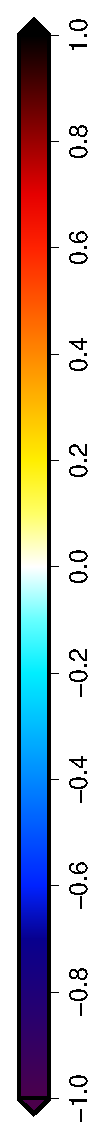
\includegraphics[height=5in,angle=270]{legends/thetaDiffWide.eps}
%
	\caption{Potential temperature anomalies of terrain following advection of a stable potential temperature profile at $t = \SI{18000}{\second}$.}
	\label{fig:wobblyThetaAdvection:thetaDiff}
\end{figure}

\begin{table}
\centering
\begin{tabular}{ r @{\hspace{2em}} l l l l l l l l}
\toprule
			& \multicolumn{3}{c}{Gravity waves, $h_0 = \SI{250}{\meter}$}	& \multicolumn{3}{c}{Gravity waves, $h_0 = \SI{500}{\meter}$}	& \multicolumn{2}{c}{Thermal profile advection} \\
Height (\si{\meter})	& BTF	& SLEVE	&	SnapCol	& BTF	& SLEVE	& SnapCol & BTF & SnapCol \\ \midrule
150 & \num{-0.003} & \num{-0.001} \\
450 & \num{0.006}  & \num{0.013} \\
750 & \num{0.032}  & \num{0.03} \\
1050 & \num{0.046} & \num{0.04} \\
\bottomrule
\end{tabular}
%
\caption{\TODO}
\label{fig:theta-sample}
\end{table}


\chapter{Conclusions}
\label{sec:conclusions}

This project has compared BTF and SLEVE terrain following grids with a cut cell style grid by analysing the numerical errors of results from a finite volume model of the fully-compressible Euler equations across five, two-dimensional test cases.

The model's upwind-biased cubic advection scheme, introduced in section~\ref{sec:method:discretisation} was tested in the horizontal and terrain following advection of a tracer (sections~\ref{sec:advection} and \ref{sec:wobblyTracerAdvection} respectively).  Results of horizontal advection preserved tracer shape on all grids and tracer magnitude was well-preserved on all except the BTF grid.  Results on the SnapCol grid were comparable to those on a regular grid without orography.  Errors were largest on the BTF grid, with artefacts remaining above the mountain, and mild distortion as the tracer passed over the mountain, though accuracy was nevertheless better than BTF result from \textcite{schaer2002}.  Conversely, errors on the BTF grid were greatly reduced in the terrain following tracer advection, but the result on the SnapCol grid was the worst of all the tracer advection tests with tracer magnitude significantly reduced.  Improvements to the advection scheme are suggested in section~\ref{sec:further-work:advection}.

In the resting atmosphere test presented in section~\ref{sec:resting}, spurious vertical velocities on the SLEVE grid were comparable to the same result from \textcite{schaer2002}, but offered only a small improvement compared to the BTF grid.  Vertical velocity was reduced by almost three orders of magnitude on the SnapCol grid.  Spurious velocities on the regular grid were still higher than the result on a cut cell grid from \textcite{good2013}, and this is the subject of further work in section~\ref{sec:further-work:resting}.

Energy was well-conserved on all grids with energy slowly decreasing on the SnapCol grid and a regular grid with flat terrain.  However, periods of energy gain were found on BTF and SLEVE grids which require further work to diagnose.

In section~\ref{sec:gw}, orographically induced gravity waves were modelled.  Velocity fields were qualitatively very similar across all grids, and vertical velocity contours agreed with the mass-conserving semi-implicit semi-Lagrangian result from \textcite{melvin2010}.  Little evidence of the `small cell' problem was found and we argued that, because the flow was mainly horizontal, this had negligible effect on the Courant number in thin cells.

Potential temperature anomalies in the gravity waves test were also visually similar, except near the ground in the lee of the mountain on the SnapCol grid.  Potential temperatures were anomalously high in the lowest layer, and anomalously low in the layer immediately above.  This is a typical manifestation of the Lorenz computational mode in which discrete hydrostatic balance is preserved despite a `zig-zag' in potential temperature.
The magnitude of these anomalies increased on the SnapCol grid when the mountain height was doubled, but results on the TF grids were largely unaffected.

A final test was designed to investigate the cause of these potential temperature anomalies (section~\ref{sec:wobblyThetaAdvection}.  We hypothesised that errors in the advection scheme excited the Lorenz computational mode.  The same stable thermal profile was advected using a terrain following velocity field that imitated the velocity field in the gravity waves test.  Once again, potential temperature anomalies were found in the lowest two layers in the lee of the mountain.  However, in this advection test, the anomalies were reversed with the anomalously low potential temperatures in the lowest layer.  It is possible that the structure of errors differ because the velocity fields in the gravity waves test and the thermal advection test were not the same.  Further tests are required to be certain of the cause of the Lorenz computational mode, and this is discussed in section~\ref{sec:further-work:gw}.

\chapter{Further work} \label{sec:further-work}
The results of the five experiments from chapter~\ref{sec:results} motivate several routes of further work.  Before discussing these, however, we identify three other items worthy of study.

First, in order to compare results with those from other experiments, such as \textcite{good2013}, the SnapCol grid should be improved so that all cut cells are aligned in rows and columns.  As discussed in section~\ref{sec:method:grid}, some cells that intersect the surface are slightly distorted during the construction of the SnapCol grid.

Second, all experiments were performed on in Cartesian coordinates and, unlike most existing implementations of terrain following layers, no coordinate transform was used.  We should investigate the metric terms introduced by terrain following coordinates, and determine whether a discretisation with metric terms can be mathematically equivalent to the Cartesian coordinate discretisation.

Third, it is desirable to perform additional verification of the model of \textcite{weller-shahrokhi2014} using idealised simulations on regular grids without orography.  Following the set of test cases for nonhydrostatic models proposed by \textcite{skamarock2004}, two further tests might be undertaken.  First, following \textcite{skamarock-klemp1994}, a simulation of the evolution of gravity waves from a potential temperature anomaly in a stable atmosphere with a horizontal wind.  Second, following \textcite{straka1993}, a cold bubble sinks to the ground, creating a density current that travels horizontally.  Results of both tests should be compared with reference solutions from \textcite{skamarock-klemp1994} and the results of \textcite{jebens2011}.

\section{Advection scheme}
\label{sec:further-work:advection}

For the three advection tests described in sections~\ref{sec:advection}, \ref{sec:wobblyTracerAdvection} and \ref{sec:wobblyThetaAdvection}, the standard OpenFOAM advection solver was used, which has two shortcomings.  First, whilst advection is treated explicitly in the fully-compressible model from \textcite{weller-shahrokhi2014}, the scalar transport model solves the advection equation (equation~\ref{eq:advection:continuous}) using implicit time-stepping.  Second, the velocity fields for the three advection tests had velocities stored at cell centres.  The scalar transport model introduces additional error when velocities are linearly interpolated onto cell faces during model initialisation\footnote{For details, refer to \url{https://github.com/OpenFOAM/OpenFOAM-2.3.x/blob/9fd0db/src/finiteVolume/cfdTools/incompressible/createPhi.H}}.

To avoid these two issues, a custom scalar transport model should be implemented that solves the advection equation explicitly and accepts a field in which velocities are defined at cell faces.  This has the added advantage that any velocity field from any fully-compressible simulation, such as the gravity waves test from section~\ref{sec:gw}, can be used as the prescribed velocity field for an advection test.

The upwind-biased cubic advection scheme, described in section~\ref{sec:method:discretisation}, is not monotonic.  Results from horizontal and terrain following tracer advection tests showed that minimum and maximum tracer values decreased over time (see sections~\ref{sec:advection} and \ref{sec:wobblyTracerAdvection}).
In similar tracer advection experiments, \textcite{jones2013} found that the van Leer scheme gave most accurate results.  The scheme is designed to maximise boundedness and accuracy, blending a centred difference scheme that is second-order accurate and unbounded with an upwind scheme that is first-order accurate and bounded.  This motivates the development of a monotonicity preserving version of the upwind-biased cubic advection scheme.  Due to its larger stencil size, we would expect such a scheme to have greater accuracy compared to the current upwind-biased scheme, and the van Leer scheme used by \textcite{jones2013}.

Results from horizontal and terrain following tracer advection tests also showed that accuracy was greatest when the velocity field was aligned with the grid.  This motivates further tests using an adaptive mesh that is dependent upon the flow.  An adaptive mesh redistribution technique might be employed such as the three dimensional formulation by \textcite{browne2014}.

\section{Resting atmosphere errors}
\label{sec:further-work:resting}

Three findings from the resting atmosphere test (section~\ref{sec:resting}) have yet to be understood.  First, compared to the results of \textcite{good2013}, the maximum vertical velocity on a regular grid is larger than expected (figure~\ref{fig:resting:w:model}) which may be due to loss of precision when loading the initial conditions.
Second, computational oscillations in vertical velocity were found on the BTF grid which eventually lead to numerical instability (not shown).  This error has not been seen on any other grid, nor in any other test case.
Third, whilst total energy gradually decreased on the SnapCol and regular grids, some energy gain was seen on the BTF and optimised SLEVE grids.  Given that energy continued to increase on the BTF grid, we would expect this to contribute to the numerical instability.

Therefore, further work is required using longer integration times to diagnose the errors in this test and, in particular, more effort is needed to understand the lack of energy conservation.  Additionally, two more resting atmosphere tests should be carried out.  First, the mountain height should be increased from \SI{1}{\kilo\meter} to \SI{4}{\kilo\meter} for comparison with results from \textcite{zaengl2012} and \textcite{good2013}.  Second, a test of a neutrally stable atmosphere at rest by \textcite{botta2004} found that errors were close to machine precision but that errors increased when stratification was included.  Comparisons with this test would be useful to further explore the sources of numerical error in idealised resting atmospheres.

\section{Gravity waves and potential temperature errors}
\label{sec:further-work:gw}

The results of terrain following advection of a stable thermal profile (section~\ref{sec:wobblyThetaAdvection}) showed a different potential temperature error structure compared to those on the SnapCol grid in the gravity waves test (section~\ref{sec:gw}).  These results could be different because the velocity fields in the two tests are not the same.

Instead of a prescribing an idealised velocity field, a further advection test might be developed that uses a velocity field more similar to the gravity waves simulation.
The gravity waves velocity field on the BTF grid might be taken as the prescribed velocity field in the new advection test.  The custom transport model, discussed earlier in this chapter, would make this straightforward on the BTF grid.  However, velocities would have to be interpolated from the BTF grid onto the SnapCol grid.  We could not simply prescribe the SnapCol velocity field from the gravity waves test because the velocity field itself may contain errors.

By using a more physical velocity field we hope that the new advection test would produce the same potential temperature error structure as the errors on the SnapCol grid in the gravity waves test.  This result would confirm that the Lorenz computational mode is excited by errors in the advection of potential temperature.

To further investigate the Lorenz computational mode found on the SnapCol grid in the gravity waves test, a Charney--Phillips staggering should be formulated and implemented for unstructured grids.  We hypothesise that the potential temperature errors near the ground on the lee slope would be reduced on a Charney--Phillips grid since stationary oscillations in the potential temperature field would not be maintained.

Little evidence of the small cell problem was found in the gravity waves test.  The Courant number was shown to be independent of horizontal velocity and, because flow is near-horizontal in the gravity waves test, there was no small cell problem.  To confirm this hypothesis, another test might be constructed in which a cold thermal anomaly descends onto a mountain.  This test is similar to density current from \textcite{straka1993} but includes a mountain profile.  The vertical momentum that reaches the surface should, for a sufficiently large timestep, cause numerical instability on the SnapCol grid but a stable solution on terrain following grids.  This would motivate the merging of small cells following \textcite{yamazaki-satomura2010}.

All tests presented in this project use one of two wave-shaped mountain profiles (given by equations~\ref{eqn:advection:schaerCos} and \ref{eqn:resting:mountain}).  Many experiments on cut cell grids perform simulations over bell-shaped mountain profiles known as `Witch of Agnessi' \parencites{steppeler2002}{rosatti2005}{klein2009}{jebens2011}.  Following \textcite{gallus-klemp2000}, a further test should be developed to simulate flow over a the bell-shaped mountain profile to allow comparison with existing results.

\textcite{lock2012} extended the two-dimensional test from \textcite{gallus-klemp2000} to simulate flow over a three dimensional mountain, presenting results on a cut cell grid.  It would be valuable to compare model results for terrain following and cut cell grids in three dimensions.


\backmatter
\printbibliography

\end{document}
